\chapter{Local Fourier Spectral Filters}
%We propose the use of Local Fourier-Spectral (LFS) filters, developed originally for 1-D and 2-D tensor-product elements by Asthana and López-Morales [cite], as a parameter-free approach to stabilize high-order solutions. The LFS filters stabilize the solution, when needed, under all potential modes of failure. Their formulation adapts easily to Finite-Element-based spatial discretizations: the filter has a compact stencil, is not more expensive than a solution evaluation, and is discretization-agnostic. We present solutions to turbulent, transonic, and supersonic flows using the Flux Reconstruction approach, a high-order scheme heavily studied in the Aerospace Computing Laboratory. All solutions are obtained in coarse, unstructured grids using a medium-cost multi-GPU-powered workstation.
%
%\subsection{Introduction}
%Mention that author was seeking filters that could be posed as a matrix-vector multiplication with a local stencil. Inspiration came from paper by Lodato.
%
%\subsection{Non-linear stabilization of high-order Flux Reconstruction schemes}
%Present summary of paper by Asthana et al. and key results.
%
%\subsection{1-D and 2-D tensor product element filtering approach}
%Describe original approach by Asthana et al. to filtering: basis functions outside element of interest are defined as constants in 1-D, and extruded curves and constants in 2-D.
%
%\subsection{Extension to arbitrary elements}
%Describe how filtering matrix is composed of two submatrices: square matrix that modifies the spectrum (energetic content) of the solution, and rectangular matrix that ensures the filter is Essentially Local Extremum Diminishing.
%
%The formulation of this type of filter is agnostic to the type of element and basis functions used, and provides a framework to design new LFS.
%
%\subsection{Simulations}
%\subsubsection{1D}
%\subsubsection{2D}
%\subsubsection{3D}

\section{Introduction}
Low-order methods are ubiquitous in industry and academia. Regardless of the mesh quality and flow conditions, commercial \gls{cfd} packages output an answer. It is up to the informed user to decide if such answer is believable or accurate to her satisfaction. This is not so true of high-order methods: they are still sensitive to starting conditions, mesh quality, and the non-linearity of the flow, i.e. how high \gls{re} is. If any of these parameters is not chosen well, the simulation will halt prematurely and no result, not even a rough estimate, will be provided. Certainly, this is not acceptable in an industrial setting.

The \gls{lfs} filters being proposed in this chapter are an attempt at tackling the low robustness of high-order methods from the perspective of flow physics, rather than the classical frameworks of polynomial order reduction, artificial viscosity, or limiting. Very promising results have been shown by Asthana and the author~\cite{asthana2014} for 1D non-linear advection-diffusion problems and 2D inviscid high-\gls{ma} flows with quadrilateral, unstructured, coarse grids, and polynomial discretizations of up to order $8$. The present paper extends their formulation to arbitrary elements in arbitrary dimensions and shows results in high-\gls{re} flows without turbulence modeling.

It is well known that turbulent flows --which tend to be high-\gls{re}--, exhibit an energy cascade: the energy from large scales is transferred to smaller scales due to natural dissipation. In very crude terms, large vortices become ever smaller vortices until they reach dimensions proportional to the Kolmogorov length-scale~\cite{kolmogorov1962refinement}. This phenomenon is well captured by the \gls{ns} equations. Hence, a good \gls{ns} solver would see large scales become ever smaller. In general, low-order methods in grids not created for \gls{dns} introduce enough numerical dissipation that the ever shrinking scales are dissipated before they become aliased (or under-sampled).

We postulate that it is precisely this very natural energy cascade which is de-stabilizing high-order numerical methods. Because high-order methods introduce little numerical dissipation, the ever shrinking scales may not be dissipated before they become aliased: they re-appear as larger scales that, naturally, become smaller later on. This vicious cycle introduces non-physical energy into the flow until the simulation is de-stabilized. Thus, removing the small scales before they become aliased would, in theory, stabilize the solution.

\gls{lfs} filters target scales relative to the element size, as the filtering operation happens in the reference element. The smaller the element, the smaller the scale being filtered. In addition, the filters help satisfy boundary conditions. The  results presented here show that the \gls{lfs} filters can  stabilize not only high-$\Re$ flows but also moderate-$\Ma$ and low-$\Ma$ flows in coarse grids, which opens the door to using the filters as pre-conditioners or in multigrid cycles. All simulations being presented ran from start to finish without intervention.

Many stabilization schemes created for high-order methods have focused on shock-capturing. A concise review of the shock-capturing literature can be seen in Section 3.4 in~\cite{vincent2011facilitating}. An \gls{av}-based shock capturing approach that has gained popularity because of its ease of implementation and increase of robustness was suggested by Persson and Peraire~\cite{persson2006sub}. A similar approach for high-$\Re$ flows with turbulence modeling has been proposed by Nguyen et al.~\cite{nguyen2007rans}. Lodato~\cite{lodato2014structural} has used filtering in the formulation of \gls{sgs} models for \gls{les} with high-order \gls{sd} schemes. His work inspired the formulation of the filters presented here. A stabilization strategy based on optimization was suggested by Guba et al.~\cite{guba2014optimization} shows great promise. A limiter-based stabilization strategy easily implemented in \gls{dg}-type methods was proposed by Kuzmin~\cite{kuzmin2004high} and Lv et al.~\cite{lv2015entropy}.

The main reason we decided to find a stabilization strategy that could be posed as a matrix multiplication and requires a very local stencil arises from the fact that \gls{hf} performs best on \gls{gpu}s. \gls{gpu}s require a low-communication, highly-parallel implementation with organized memory accesses and homogeneous computations. Implementation of \gls{av} would have required elements adjacent to each other to share information about the \gls{av} that each requires, leading to inevitable additional inter-element communication.

 Section \ref{sec:frmethod} presented a general description of the \gls{fr} method. Section \ref{sec:extension_multiple_dimensions} showed how this scheme relies on matrix multiplications and, hence, a filter that costs two small matrix multiplications per element is ideal for \gls{fr}. Section \ref{sec:lfsfilter} describes the properties being sought in the \gls{lfs} filters and the mechanics of their implementation. Section \ref{sec:visualization} provides visualizations of the filters and their effects on a polynomial solution. Section \ref{sec:results} presents the results of 2D simulations, in unstructured coarse grids, of flows where \gls{re}$= 1e6$. This \gls{re} number was selected because of the availability of experimental data for the case of the circular cylinder and \gls{hf} had not been run at these \gls{re} numbers. In addition, Section \ref{sec:filteringEffects} shows results that isolate the effects of filtering from the effects of coarsening a grid or changing the spatial order of accuracy to demonstrate that \gls{lfs} filters preserve element-wise spectral properties.


\vspace{.20in}



\vspace{.20in}

\section{Local Fourier Spectral Filters}
\label{sec:lfsfilter}

\subsection{Desired Properties}
\label{sec:lfs_properties}
When designing the \gls{lfs} Filters presented in this paper, we considered the following properties as desirable:
\begin{enumerate}[1. ]
\item The filter should have spectral interpretation so there is control over the physical scales being smoothed
\item \label{item:local_stencil} The filtering operation must have a local stencil: only interior and boundary solution values can be used to filter the solution in the interior of the element
\item \label{item:filt_bc}The filter should preserve boundary conditions
\item \label{item:filt_bi}Filtering the solution at the interior points should be influenced by the solution values at the element's boundary
\item \label{item:influence}The influence of a boundary point on the internal point being filtered should be inversely proportional to the distance between them
\item To limit computational cost, the filter should be applied in the reference domain and involve matrix-vector multiplications exclusively

\item \label{item:generalizability}Filtering strategy should be generalizable to any type of element in unstructured grids

In the early stages of the filter design, we noted that Properties \ref{item:filt_bc} and \ref{item:filt_bi} could be overly stringent, so we re-phrased them as the following, more relaxed condition:

\item \label{item:coplanar}If solution values at the boundary lie on a hyperplane in the space of spatial coordinates and solution values, the filtering operation should bring the internal solution values closer to such plane. In other words, if the solution values at the boundaries can be determined from a linear function of their location, the filter should bring the internal solution values closer to satisfying such linear function.
\end{enumerate}



Condition \ref{item:coplanar} may not allow a filtered solution to satisfy the boundary conditions always. Nevertheless, in the limit of infinite mesh refinement the solutions at the boundary of every element will be coplanar, even in the presence of shocks in the \gls{ns}  equations. Hence, Condition \ref{item:coplanar} satisfies conditions \ref{item:filt_bc} and \ref{item:filt_bi} asimptotically. This re-formulation was inspired by the \gls{eled}  property of the \gls{jst}  scheme\cite{jameson1981numerical} for finite volume methods. Whether or not (some) \gls{lfs} filters satisfy \gls{eled}  properties shall be left for a future study.

%At this point it is important to note the main difference between the filters being proposed here and the commonly used modal filters\cite{kanevsky2006idempotent}. Modal filters are not influenced by the values of the solution at the boundary points. Therefore, if an element is experiencing aliasing, a modal filter will not necessarily ``nudge" the internal solution values towards continuity with its neighbors. In addition, in the limit of mesh refinement, modal filtering might not enforce an element's boundary conditions.

\subsection{Mechanics of \gls{lfs} Filters}

The core idea of the \gls{lfs} filtering technique is that the solution is filtered with a matrix whose entries depend on the element interface values, the basis functions of the solution, and a selected Fourier filtering kernel.

Suppose we wish to filter the scalar field $v$ inside an arbitrary element. This field could be density, momentum in a specific direction, or energy. We can represent $v$, as usual, as a weighted sum of basis functions.
\begin{equation}
\label{eqn:polyexp}
v(\bxi) = \sum^{N_s}_{i=1} v_i \phi_i(\bxi),
\end{equation}
where $v_i$ is the \ith weight, $\bxi$ is a vector of coordinates in a reference domain, and $\phi_i(\bxi)$ is the \ith basis function.

The key component of the \gls{lfs} technique is that the Fourier filtering operation over the element is approximated at each internal point $i$ with coordinates $\bxi_i$. Suppose we wish to use filtering kernel $G(\bxi)$ to filter $v(\bxi)$, then the filtered value at internal point $i$ becomes
\begin{equation}
\label{eqn:convolution}
\begin{split}
\bar{v}_j &= (G \ast v)(\bxi_j)\\
&= \int_{\mathbb{R}^d} G(\bxi_j - \bxi)v(\bxi)d\bxi\\
&= \int_{\mathbb{R}^d} G(\bxi_j - \bxi)\l(\sum^{N_s}_{i=1} v_i \phi_i(\bxi)\r)d\bxi\\
&= \sum^{N_s}_{i=1}v_i\int_{\mathbb{R}^d} G(\bxi_j - \bxi)  \phi_i(\bxi)d\bxi,\\
\end{split}
\end{equation}

where $\Omega$ is the entire problem domain, not just the element domain, $N_s$ is the number of solution points, and the overbar means the quantity is filtered. Filtering over the entire domain would be computationally expensive, but would certainly smoothen the solution field and can be done while maintaining the order of accuracy of the underlying numerical scheme\cite{mirzaee2012efficient,steffen2008investigation,walfisch2009one}. In order to use only a local (element-wise) stencil, it is possible to break the integration as follows
\begin{equation}
\label{eqn:brokenint}
\int_{\mathbb{R}^d} G(\bxi_j - \bxi)  \phi_i(\bxi)d\bxi = \int_{\Omega_n} G(\bxi_j - \bxi)  \phi_i(\bxi)d\bxi + \int_{\mathbb{R}^d \backslash \Omega_n} G(\bxi_j - \bxi)  \phi_i(\bxi)d\bxi,
\end{equation}
where $\Omega_n$ is the domain of element $n$ (where the $\phi_i$ values are known) and $\Omega \backslash \Omega_n$ is the complement of $\Omega_n$ in $\Omega$. As $G$ and $\phi_i$ are defined in $\Omega_n$, it is possible to calculate the first integral in Equation \eqref{eqn:brokenint} analytically or via an adaptive quadrature algorithm like \texttt{quanc8}~\cite{forsythe1977computer}.

A design choice arises in defining $\phi_i$ in the domain $\Omega \backslash \Omega_n$. Asthana et al.~\cite{asthana2014} initially decided to let $\phi_i$ equal a constant in 1D elements, and a combination of constant and polynomial in quadrilaterals. Non-tensor-product elements became problematic for this kind of formulation. This paper presents a more generic filter design method based on the desired properties in Section \ref{sec:lfs_properties}.

Let us describe the mechanics of the two components of the integral in Equation \eqref{eqn:brokenint} in a subsection each. We can call the filter associated with the term $\int_{\Omega_n} G(\bxi_j - \bxi)  \phi_i(\bxi)d\bxi$ ``Internal Filtering Component" and the filter associated with the term $\int_{\mathbb{R}^d \backslash \Omega_n} G(\bxi_j - \bxi)  \phi_i(\bxi)d\bxi$ ``Boundary Filtering Component".

The filtering operation being sought follows this format
\begin{equation}
\label{eqn:filter_form}
\vec{\bar{v}} = \alpha\mat{T}\vec{v} + (1-\alpha)\mat{B}\vec{v^*},
\end{equation}
where $\mat{T}$ is the internal filtering component, as it acts on the solution at internal points $\vec{v}$, and $\mat{B}$ is the boundary filtering component, as it acts on the solution at boundary points $\vec{v^*}$, and $\alpha$ is a scalar between $0$ and $1$ that determines the relative influence the internal and boundary components have on the internal solution values.

\subsection{Internal Filtering Component}
There are two steps to the creation of the internal filtering component $\mat{T}$. First we create the filtering matrix with the spectral interpretation, and then we normalize it so if the quantity being filtered is a constant, the filter preserves the constant.
\subsubsection{Matrix formation}
It can be seen from the last line in Equation \eqref{eqn:convolution} that finding the vector of solution values filtered with the internal component can be posed as a matrix-vector multiplication:
\begin{equation*}
\label{eq:internal_matrix}
\begin{bmatrix}
\bar{v}_1 \\
\bar{v}_2 \\
\vdots\\
\bar{v}_{N_s} \\
\end{bmatrix} = 
\begin{bmatrix}
\int_{\Omega_n} G(\bxi_1 - \bxi)  \phi_1(\bxi)d\bxi &
\int_{\Omega_n} G(\bxi_1 - \bxi)  \phi_2(\bxi)d\bxi &
\cdots &
\int_{\Omega_n} G(\bxi_1 - \bxi)  \phi_{N_s}(\bxi)d\bxi\\
\int_{\Omega_n} G(\bxi_2 - \bxi)  \phi_1(\bxi)d\bxi &
\int_{\Omega_n} G(\bxi_2 - \bxi)  \phi_2(\bxi)d\bxi &
\cdots &
\int_{\Omega_n} G(\bxi_2 - \bxi)  \phi_{N_s}(\bxi)d\bxi\\
\vdots & \vdots & \ddots & \vdots\\
\int_{\Omega_n} G(\bxi_{N_s} - \bxi)  \phi_1(\bxi)d\bxi &
\int_{\Omega_n} G(\bxi_{N_s} - \bxi)  \phi_2(\bxi)d\bxi &
\cdots &
\int_{\Omega_n} G(\bxi_{N_s} - \bxi)  \phi_{N_s}(\bxi)d\bxi
\end{bmatrix}
\begin{bmatrix}
v_1 \\
v_2 \\
\vdots\\
v_{N_s} \\
\end{bmatrix}.
\end{equation*}

More compactly,
\begin{equation}
\label{eqn:filtmat}
\vec{\bar{v}} = \mat{F}\vec{v}
\end{equation}
we use over-arrow to denote column vectors.
Interesting choices for $G(\bxi)$ depend on a desired wavenumber threshold $h$:

\begin{enumerate}[I.]
\item Gaussian function:
$$
G(\bxi) = h \exp{(h||\bxi||)},
$$
where $||\bxi||$ is a measure of the length of $\bxi$.
\item \label{item:multi_ind_func}Multidimensional indicator function:
$$
G(\bxi) = h\mathrm{I}_{[0,1]}(h||\bxi||),
$$
where $\mathrm{I}_{[0,1]}(x) = 1 \text{ if } 0\le x\le 1$, and $0$ otherwise.
\item \label{item:sharp_spectral}Multidimensional sharp-spectral function:
$$
G(\bxi) = h||\bxi||^{-n/2}
J_{n/2}(h||\bxi||),
$$
where $J_\alpha$ is a Bessel function of the first kind and $n$ is the number of dimensions of $\bxi$.
\end{enumerate}

In these functions, the larger the value of $h$, the thinner the filter is in physical space, so the fewer wavenumbers it dampens. Note that as $h \rightarrow \infty$, $\mat{F}_{ij}  \rightarrow \phi_j(\bxi_i)$, so $\vec{\bar{v}} \rightarrow \vec{{v}}$. The integrals in Equation \eqref{eq:internal_matrix} can be evaluated to arbitrary accuracy with \texttt{quanc8}~\cite{forsythe1977computer} in a pre-processing stage.

\subsubsection{Enforcing Conservation of a Constant Quantity}
The requirement to preserve a constant can be posed in an equation as
\begin{align}
\bar{v}_i = \sum^{N_s}_{j = 1} \mat{F}_{ij} v_{\text{const}} = v_{\text{const}},
\end{align}
where $v_{\text{const}}$ is a constant scalar. As a result, each row of $\mat{F}$ must satisfy
\begin{align}
\sum^{N_s}_{j = 1} \mat{F}_{ij} = 1,
\end{align}
where $i = 1,\dots,N_s$.
This constraint can be enforced by dividing each row of $\mat{F}$ with the total sum of the row. More explicitly,
\begin{align}
{\mat{T}}_{ij} = \frac{\mat{F}_{ij}}{\sum^{N_s}_{k = 1} \mat{F}_{ik}},
\end{align}
where the normalized matrix ${\mat{T}}$ is the internal filtering component in Equation \eqref{eqn:filter_form}.

\subsubsection{Integration Domain}

The normalization of the matrix introduces a bias. As the integration is being performed in some reference domain $\Omega_n$, the integral $\int_{\Omega_n} G(\bxi_i - \bxi)  \phi_j(\bxi)d\bxi$ will tend to have a greater value when $\bxi_i$ is well inside the reference element. This is more evident when using the multidimensional indicator function (shown in \ref{item:multi_ind_func}) as the filtering kernel.

To ameliorate this bias, we have selected to perform the integration in a reference domain that is symmetric. With this precaution all integrals related to points close to a domain edge have a similar magnitude, and thus the filtering operation does not favor points close to some arbitrary edge over the others.

Figure \ref{fig:domain_example} illustrates the potential introduction of bias in triangular elements that use a right triangle as a reference element.

\begin{figure*}

\subfloat[Equilateral triangle domain\label{fig:equi_tri_domain}]{%
      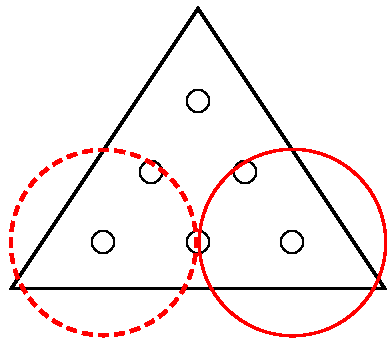
\includegraphics[width=0.45\textwidth]{\lfsdir/figs/equi_tri.pdf}
    }
    \hfill
    \subfloat[Right triangle domain\label{fig:right_tri_domain}]{%
          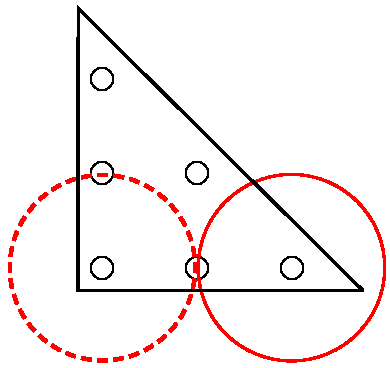
\includegraphics[width=0.45\textwidth]{\lfsdir/figs/right_tri.pdf}
        }
\caption{Using the same filter width in two different domains introduces different bias. The small, solid circles represent the location of solution points. The large circles represent the filter width acting on two specific internal points in two different domains. Integration is being performed in the area encompassed by the solid, straight lines.}
\label{fig:domain_example}

\end{figure*}

In practice, the basis functions $\phi_j(\bxi)$ may be defined in non-symmetrical elements. To simplify the evaluation of the integral, the definition of the norm in the filtering kernel $G(\bxi)$ can be modified so the curve drawn by $||\bxi -\bxi_0|| = 1$ in the non-symmetric reference element would map to a circle in a symmetric reference element.

In the case of a triangle, the basis functions are defined in a right triangle with vertices $[-1,-1], [1,-1],[-1,1]$.

By defining the norm in this right triangle as follows
\begin{equation}
\label{eqn:rect_norm}
||\bxi||^2_{rt} = \bxi_1^2 + \bxi_2^2 + \bxi_1\bxi_2,
\end{equation}
$||\bxi -\bxi_0||_{rt} = 1$ maps to a circle in the equilateral triangle with vertices $[-1,-1],[1,-1],[0,\sqrt{3}-1]$. Figure \ref{fig:mapping} sketches this mapping. $||\cdot||_{rt}$ is the norm defined in the right triangle.


\begin{figure}\centering
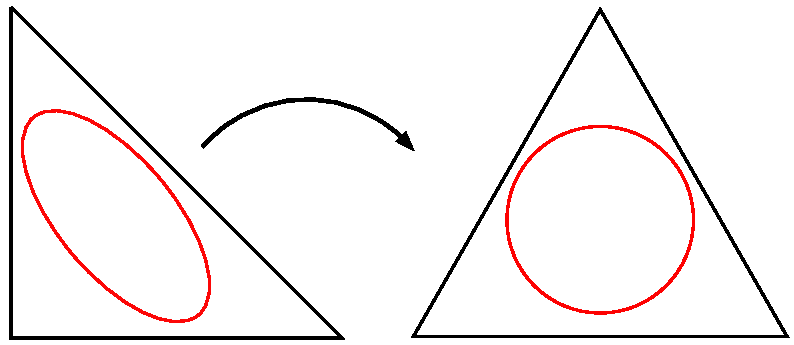
\includegraphics[width = 0.75\textwidth]{\lfsdir/figs/mapping.pdf}
\caption{Sketch of ellipsis $||\bxi -\bxi_0||_{rt} = 1$ defined in the right triangle domain maps to a circle in the equilateral triangle domain}
\label{fig:mapping}
\end{figure}

\subsection{Boundary Filtering Component}

Formulating the influence of boundary solution values on internal solution values as a matrix is not so straightforward. The approach being suggested here is based on some reasonable desired properties, but some choices are arbitrary. 

The creation of this matrix proceeds as follows: place the boundary points and the internal points in a symmetric domain, select an ``influence" function with as many unknowns as dimensions, find values for these unknowns such that Condition \ref{item:coplanar} is satisfied, and create the boundary filtering component.

\subsubsection{Ensuring Boundary Filtering Component Preserves Linearity of the Solution at the Boundary (Condition \ref{item:coplanar})}
In this sub-section, we seek to form matrix $\mat{B}$ in Equation \ref{eqn:filter_form}. In this analysis, we assume that $\alpha = 0$ in Equation \ref{eqn:filter_form} so we can isolate $\mat{B}$'s properties from those of $\mat{T}$.

The preservation of linearity can be posed in the following way. Assume that values $\vec{v^*}$ at the boundaries are linear in space. More explicitly, for each boundary point $i = 1,\dots,N_f$
\begin{equation}
v^*_i = {\bxi^*_i}^\mathrm{T}\vec{a} + b,
\end{equation}
where $v^*_i$ is the solution at the \ith boundary point, $\bxi_i^*$ are the coordinates of such boundary point, $\vec{a}$ is a vector of constant coefficients, and $b$ is a constant scalar. In vector notation, we are assuming

\begin{equation}
\label{eq:linear}
\vec{v^*} = \underline{\bxi^*}^\mathrm{T}\vec{a} + \vec{b^*},
\end{equation}
where $\vec{b^*} = b\mathbbm{1}_{[N_f \mathrm{x} 1]}$ and $\underline{\bxi^*}^\mathrm{T}$ is a matrix of dimensions $N_f$ by $N_d$ --number of dimensions.

To satisfy Condition \ref{item:coplanar}, we seek a matrix $\mat{B}$ such that, when $\vec{v^*}$ satisfies Equation \ref{eq:linear},
\begin{equation}
\vec{\bar{v}} = \mat{B}\vec{v^*} = \underline{\bxi}^\mathrm{T} \vec{a} + \vec{b},
\end{equation}
where $\vec{b} = b\mathbbm{1}_{[N_s \mathrm{x} 1]}$ and $\underline{\bxi}^\mathrm{T}$ is a matrix of dimensions $N_s$ by $N_d$. The \ith row of $\underline{\bxi}^\mathrm{T}$ is ${\bxi_i}^\mathrm{T}$, the coordinates of the \ith internal point.

Therefore, we seek a matrix $\mat{B}$ such that
\begin{equation}
\mat{B}\l(\underline{\bxi^*}^\mathrm{T}\vec{a} + \vec{b^*}\r) = \underline{\bxi}^\mathrm{T} \vec{a} + \vec{b}.
\end{equation}

As a result, for general $ \underline{\bxi^*}^\mathrm{T}$, $\underline{\bxi}^\mathrm{T} $, and $\vec{a}$,
\begin{align}
\mat{B}\underline{\bxi^*}^\mathrm{T} = \underline{\bxi}^\mathrm{T}  \hspace{1cm} &\text{and} \hspace{1cm} \mat{B}\vec{b^*} = \vec{b}\\
\label{eqn:Bconditions}\implies \hspace{1cm} \sum_{j=1}^{N_f}\mat{B}_{ij}\xi^*_{jd} = \xi_{id} \hspace{1cm} &\text{and} \hspace{1cm} \sum_{j = 1}^{N_f} \mat{B}_{ij} = 1
\end{align}
for all $i = 1,\dots,N_s$ and $d = 1,\dots,N_d$. Where $\xi^*_{jd}$ is the $d^\text{th}$ coordinate of the $j^\text{th}$ boundary point, and $\xi_{id}$ is the $d^\text{th}$ coordinate of the $i^\text{th}$ internal point.

Equation \ref{eqn:Bconditions} introduces $N_s (N_d + 1)$ constraints for $N_sN_f$ unkonwns in $\mat{B}$. Each row in $\mat{B}$ needs to satisfy $N_d+1$ equations. Table \ref{tab:conds_unknowns} shows the number of equations and unknowns for specific elements assuming that the solution whithin each is represented by a polynomial of degree $p\ge0$.

\newcommand{\len}{0.6cm}

    \begin{table}

    \cellspacebottomlimit=5pt
    \cellspacetoplimit=5pt
%      \begin{center}
        \newlength{\oldtabcolsep}                 % keep track of old \tabcolsep
        \setlength{\oldtabcolsep}{\tabcolsep}     % 6.0pt
        \setlength{\tabcolsep}{0pt}               % so coloring doesn't run off
                                                  % ends of the table
        \renewcommand{\arraystretch}{2}         % because math expressions
                                                  % almost run into each other
%        \begin{tabular}{Sl<{\hspace{2cm}}l<{\hspace{\oldtabcolsep}}l}  
\hspace{-2cm}
\begin{tabular}{l <{\hspace{\len}}c <{\hspace{0.2cm}} c <{\hspace{0.2cm}}c<{\hspace{\len}} c<{\hspace{\len}} c<{\hspace{\len}} c }

          \toprule
Element type & $N_s$& $N_d$ & $N_f$ & \specialcell[b]{\# of Equations:\\ $N_s (N_d + 1)$} & \specialcell[b]{\# of Unkowns:\\$N_sN_f$} \\
          \specialrule{\lightrulewidth}{0pt}{0pt} % so row-coloring aligns

Line & $p+1$ & $1$ & $2$ &$2(p+1)$ & $2(p+1)$\\

Triangle & $\frac{1}{2}(p+1)\cdot(p+2)$ & $2 $ & $3(p+1)$ & $\frac{3}{2}(p+1)\cdot(p+2)$ & $\frac{3}{2}(p+1)^2\cdot(p+2)$\\
Quadrilateral & $(p+1)^2$ & $2$ & $4(p+1)$ & $3(p+1)^2$ & $4(p+1)^3$\\
Tetrahedron & \specialcell[t]{$\frac{1}{6}(p+1)\cdot(p+2)$\\$\cdot(p+3)$} & $3 $ & $4\frac{1}{2}(p+1)\cdot(p+2)$ & \specialcell[t]{$\frac{2}{3}(p+1)\cdot(p+2)$\\$\cdot(p+3)$} & \specialcell[t]{$\frac{1}{3}(p+1)^2\cdot(p+2)^2$\\$\cdot(p+3)$}\\
Pyramid & \specialcell[t]{$\frac{1}{6}(p+1)\cdot(p+2)$\\$\cdot(2p+3)$} & $3 $ & \specialcell[t]{$4\frac{1}{2}(p+1)\cdot(p+2)$\\$ + (p+1)^2$}  & \specialcell[t]{$\frac{2}{3}(p+1)\cdot(p+2)$\\$\cdot(2p+3)$} & \specialcell[t]{$\frac{1}{6}(p+1)^2\cdot(p+2)$\\$\cdot(2p+3)\cdot(3p+5)$}\\
Prism & $\frac{1}{2}(p+1)^2\cdot(p+2)$ & $3 $ & \specialcell[t]{$2\frac{1}{2}(p+1)\cdot(p+2)$\\$ + 3(p+1)^2$} & $2(p+1)^2\cdot(p+2)$ & \specialcell[t]{$\frac{1}{2}(p+1)^3\cdot(p+2)$\\$\cdot(4p+5)$}\\
Hexahedron & $(p+1)^3$ & $3 $ & $6(p+1)^2$ & $4(p+1)^3$ & $6(p+1)^5$\\
          \bottomrule
        \end{tabular}
%      \end{center}
      \caption{Number of internal points $N_s$, number of boundary points $N_f$, and number of equations and unknowns in matrix $\mat{B}$ for each type of element, assuming the solution is being discretized with a polynomial of degree $p$}
      \label{tab:conds_unknowns}

    \end{table}

All elements, except for the line element, have matrices $\mat{B}$ with more unknowns than equations. This calls for a reduction of the number of unknowns in a strategic way. This is achieved by invoking Condition \ref{item:influence}: the farther away a boundary point is from an internal point, the less influential it should be.

\subsubsection{Ensuring Influence of Boundary Points on Internal Points is Inversely Proportional to their Distance (Condition \ref{item:influence})}
Given this requirement and Equation \eqref{eqn:Bconditions}, a reasonable design choice for each entry in $\mat{B}$ is:
\begin{equation}
\label{eq:bij_unmodified}
\mat{B}_{ij} = \frac{g_i\l(||\bxi_i - \bxi_j^*|| \r)^{-1}}{\sum\limits_{k=1}^{N_f}g_i\l(||\bxi_i - \bxi_k^*|| \r)^{-1}},
\end{equation}
where $\bxi_i$ is the location of the \ith internal point, $\bxi_j^*$ is the location of the \jth boundary point, and $g_i(\cdot)$ is a monotonically increasing function and $g_i(0) = 0$. The norm $||\cdot||$ is ideally defined in a symmetric element, or a reformulation of a norm in an non-symmetric element as in Equation \eqref{eqn:rect_norm}. We note that the requirement that $\sum_{j = 1}^{N_f} \mat{B}_{ij} = 1$ is immediately satisfied regardless of the exact form of $g_i(\cdot)$.

To avoid dividing by zero when $||\bxi_i - \bxi_j^*|| = 0$, we can recast Equation \eqref{eq:bij_unmodified} as
\begin{equation}
\label{eq:bij_def}
\mat{B}_{ij} = \frac{1}{1 + g_i\l(||\bxi_i - \bxi_j^*|| \r)\sum\limits_{\substack{k=1\\k \ne j}}^{N_f}g_i\l(||\bxi_i - \bxi_k^*|| \r)^{-1}}.
\end{equation}
This definition of $\mat{B}$ is now too stringent, so it is not clear if the conditions in Equation \eqref{eqn:Bconditions} are satisfied for any selection of $g_i(\cdot)$. Each row in $\mat{B}$ has $N_d$ equations left to satisfy.

By introducing $N_d$ unknowns in the definition of $g_i(\cdot)$ we can expect to satisfy the remaining $N_d$ equations per row. A choice made here is to let
\begin{equation}
\label{eqn:g_def}
g_i(x) = \sum_{d = 1}^{N_d} a_{id} x^d,
\end{equation}
where $x$ is a scalar, and $a_{id}$ are the unknowns to be found in each row $i$.

To find the values of $a_{id}$, a regular non-linear minimization function can be invoked. In this paper, we used the downhill simplex method by Nelder and Mead~\cite{nelder1965simplex}. The implementation in C++ was adapted from Jia \cite{simplexCode}. The function being minimized for each row $i$ of $\mat{B}$ is
\begin{equation}
J_i(a_{i1},\dots,a_{1N_d})=\sum_{d=1}^{N_d}\l(\sum_{j=1}^{N_f}\mat{B}_{ij}\xi^*_{jd} - \xi_{id}\r)^2,
\end{equation}
where $J_i$ is the cost function to be minimized related to row $i$. In occasions, the minimum of $J$ does not reach machine zero. However, as it will be shown in the case of triangles, $\mat{B}$ still behaves as desired.


\vspace{.30in}

\section{Visualization of the \gls{lfs} Filters in Triangular Elements}
\label{sec:visualization}
In this section we present visualizations of the effect of the \gls{lfs} filters on a polynomial solution of degree $5$ in a reference triangle.

In the plots that follow, the internal and boundary points are located as shown in Figure \ref{fig:tri_points}.
\epstopdfsetup{update}
\begin{figure}
\centering
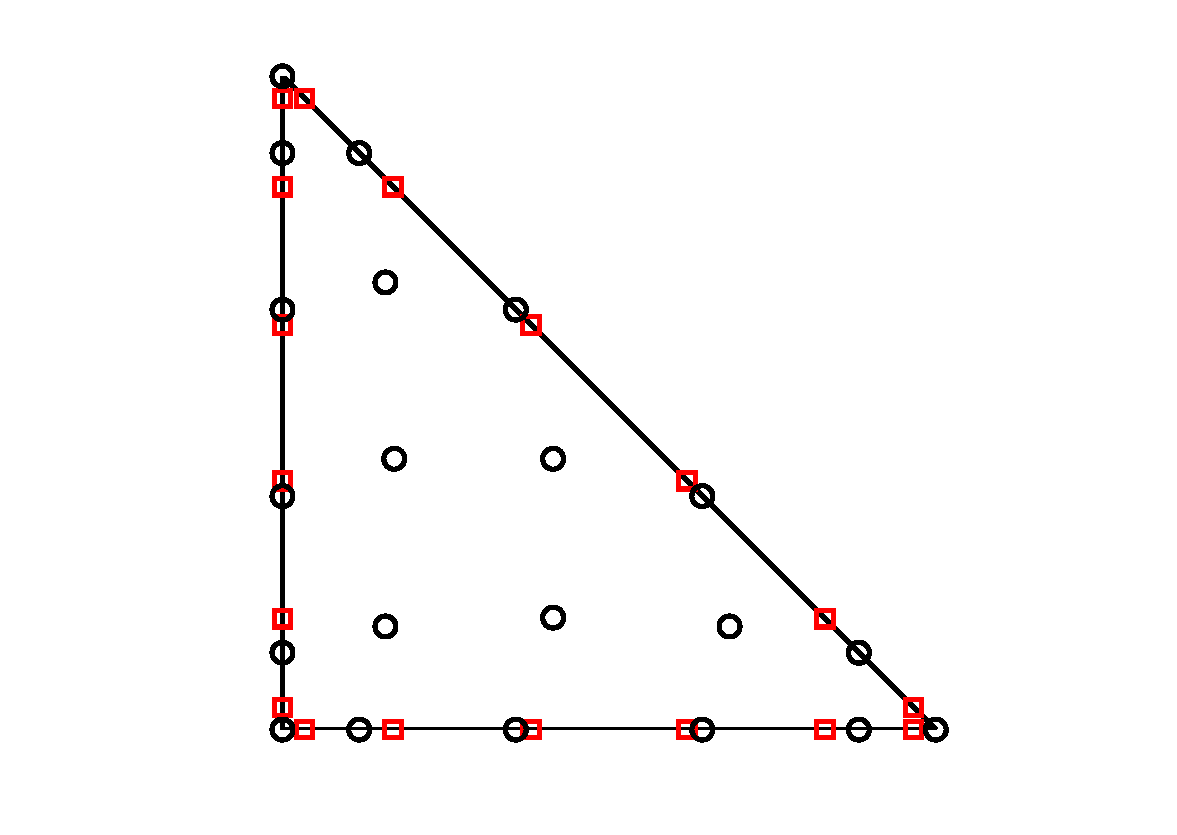
\includegraphics[width = 0.5\textwidth]{\lfsdir/figs/right_triangle_point_locations.eps}
\caption{Internal and boundary points in the reference triangular domain when solution is represented with polynomial of degree $5$ ($p=5$). Black circles represent the internal points. Red squares represent the boundary points.}
\label{fig:tri_points}
\end{figure}

\subsection{Internal Filtering Components}
To illustrate the effect of the internal filtering component, let us filter a solution using matrix $\mat{T}$ exclusively. Figure \ref{fig:internal_filt} shows the result of filtering using a width of $h=10$ in the 2-D sharp-spectral filtering kernel \eqref{item:sharp_spectral} with the modified norm \eqref{eqn:rect_norm}.
\begin{figure}
\centering
\includegraphics[width = 0.5\textwidth]{\lfsdir/figs/internal_effect.eps}
\caption{Solution values after filtering with internal component exclusively, $\vec{\bar{v}} = \mat{T}\vec{v}$, where  ${v_i} = \sin{(k\xi_{i1})} + \cos{(k\xi_{i2})} $, where $k=500$. Hollow black circles show the unfiltered solution at the interior points, transparent colored surface is the polynomial representation of the unfiltered solution, filled black circles show the filtered values of the solution at the interior points, and the meshed surface shows the polynomial representation of the filtered solution.}
\label{fig:internal_filt}
\end{figure}

It can be seen that the polynomial representation of the filtered values is smoother than the polynomial representation of the unfiltered values while maintaining the general shape and curvature.



\subsection{Boundary Filtering Components}
To illustrate the effect of the boundary filtering component, let us filter a solution using matrix $\mat{B}$ exclusively. Figure \ref{fig:boundary_effect} shows the result of filtering. Because only $\mat{B}$ is acting on the solution, the unfiltered values of the solution at the internal points are not plotted. 

We have made all the values of the solution at the boundaries co-planar to illustrate how effectively Condition \ref{item:coplanar} is satisfied. The operation of filtering with $\mat{B}$ does bring the filtered solution closer to a plane if the boundary values are co-planar.

\begin{figure}
\centering
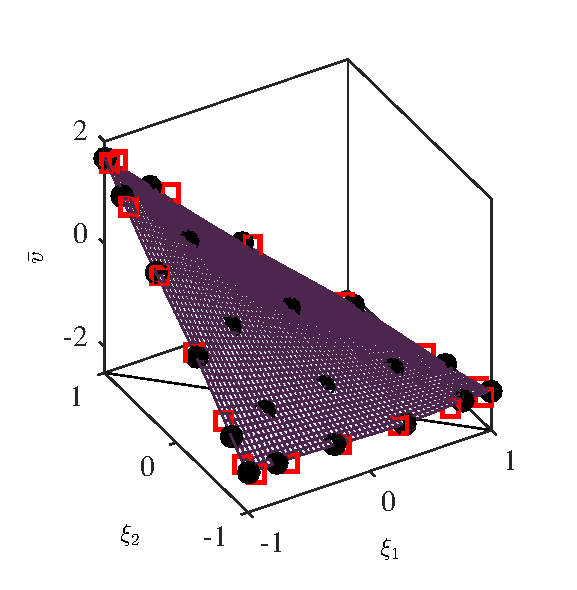
\includegraphics[width = 0.5\textwidth]{\lfsdir/figs/boundary_effect.eps}
\caption{Solution values after filtering with boundary component exclusively, $\vec{\bar{v}} = \mat{B}\vec{v^*}$, where  $\vec{v^*} = a\vec{\xi^*_1} + b\vec{\xi^*_2} + c$ for some constants $a,b,c$. Red squares show the values of the solution at the boundaries, filled black circles show the filtered values of the solution at the interior points, and the meshed surface shows the polynomial representation of the solution.} 
\label{fig:boundary_effect}
\end{figure}

Figure \ref{fig:boundary_effect_oscillatory} illustrates how the boundary filtering component would behave in the case the boundary values are not coplanar. It is interesting to note that close to the corner $(\xi_1,\xi_2) = (-1,1)$, two boundary points with different values are close to an internal point. The value  of the filtered solution close to those boundary points assumes a value that is close to the average of the two.

The polynomial interpolation of the filtered interior values shows that the closer an interior point is to a boundary point, the more it will be influenced by such boundary point. This causes the filtered values close to the boundaries to get closer to the boundary values. This suggests that the boundary filtering component does in fact help in bringing the solution closer to satisfying the boundary conditions while diminishing oscillations within the element.

\begin{figure}
\centering
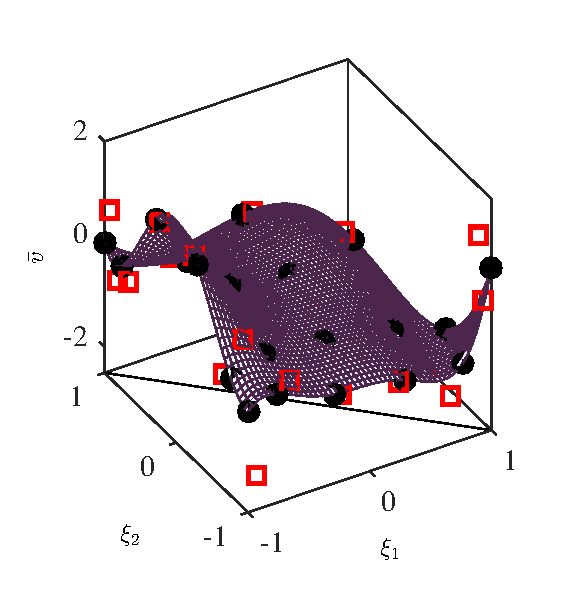
\includegraphics[width = 0.5\textwidth]{\lfsdir/figs/boundary_effect_oscillatory.eps}
\caption{Solution values after filtering with boundary component exclusively, $\vec{\bar{v}} = \mat{B}\vec{v^*}$, where   ${v_i^*} = \sin{(k\xi^*_{i1})} + \cos{(k\xi^*_{i2})} $, $k=500$. Red squares show the values of the solution at the boundaries, filled black circles show the filtered values of the solution at the interior points, and the meshed surface shows the polynomial representation of the solution.} 
\label{fig:boundary_effect_oscillatory}
\end{figure}

\subsection{Filtered Solutions}
No filtering component is used solely by itself. The factor $\alpha$ in Equation \ref{eqn:filter_form} determines how much weight to give to each component. Figure \ref{fig:filtered_solutions} illustrates the effect of the boundary values on a fully filtered solution, when $\alpha = 0.8$.

The internal filtering component reduces oscillations, while the boundary filtering component brings the interior values closer to the boundary values. By placing the boundary values on different planes, this effect becomes more evident.

\begin{figure*}
\hspace{-1cm}
\subfloat[$\beta = -0.75$\label{fig:filt_neg}]{%
\includegraphics[width=0.5\textwidth]{\lfsdir/figs/filter_tilt_neg.eps}
}
\hfill
\subfloat[$\beta = 0.75$\label{fig:filt_pos}]{%
\centering
\includegraphics[width=0.5\textwidth]{\lfsdir/figs/filter_tilt_pos.eps}
}
\caption{Solution values after filtering with both internal and boundary components, $\vec{\bar{v}} = \alpha\mat{T}\vec{v} + (1-\alpha)\mat{B}\vec{v^*}$, where $\alpha = 0.8$, ${v_i} = \sin{(k\xi_{i1})} + \cos{(k\xi_{i2})} $, $k=500$, $\vec{v^*} = \beta (-\vec{\xi^*_1} + \vec{\xi^*_2})$. Hollow black circles show the unfiltered solution at the interior points, transparent colored surface is the polynomial representation of the unfiltered solution, filled black circles show the filtered values of the solution at the interior points, hollow red squares show the value of the solution at the boundary points, and the meshed surface shows the polynomial representation of the filtered solution.}
\label{fig:filtered_solutions}

\end{figure*}
\vspace{.20in}

\section{Results}
\label{sec:results}
To test the filters' ability to increase general robustness of a high-order solver, we have implemented their formulation in \gls{hf} for triangular elements and performed simulations where the solver would become unstable otherwise.

We wanted to test the increase of robustness in extreme cases of grid coarseness, high Reynolds number, very low \gls{ma}, and moderate \gls{ma}. It is important to keep in mind that in these cases we are not seeking very accurate results, but rather robustness under all conditions. In order to popularize high-order methods, we need to make them as robust as their low-order counterparts while retaining their benefit of higher accuracy with less computational and setup effort.

The goal is to have a cheap stabilization strategy that preserves boundary conditions for cases in which the mesh is not necessarily perfectly appropriate for resolving the flow physics over the entire domain. This scenario arises frequently in industrial applications, where the mesh would be properly refined at regions of interest and coarse in regions that the engineer/scientist has decided are not as important for the problem at hand.

All the simulations that follow were performed using \gls{hf}\cite{lopez2014verification}. 2-D \gls{ns} equations are being solved, with varying values of \gls{ma}, \gls{re}, time-step ($\Delta t$), and filtering frequency. The common parameters are:
\begin{enumerate}[1.]
\item Four-stage, five-step, low-storage Runge-Kutta time-stepping method (\gls{rk45}) \cite{carpenter1994fourth} was used in the \gls{gpu}s, and forward Euler was used when running a simulation in CPUs
\item Polynomial solution representation ($p$) of order $4$. Rusanov Flux as a Riemann solver, and a \gls{ldg}~\cite{cockburn1998local} viscous flux.
\item Filters with width $h = 10$ and weghting parameter $\alpha = 0.8$.
\item Starting from uniform flow
\item Characteristic boundary conditions at the inflow and outflow. No-slip, isothermal wall boundary conditions at the cylinder's surface.
\item All quantities non-dimensionalized with free-stream temperature and cylinder wall temperature of $300$, reference length of $1$.
\item Flow properties: $\gamma = 1.4$, Prandtl number $\mathrm{Pr} = 0.72$, gas constant $R = 286.9 \frac{J}{Kg K}$, viscosity determined by Sutherland's law with reference temperature of $291.15 K$ and reference viscosity of $\mu = 1.827\mathrm{e}-5$
\end{enumerate}

Results of interest are shown in Table \ref{table:results}. Accuracy of the results is not expected. Nevertheless, as a reference, for the flow around a cylinder at \gls{re}$= 1e6$, $\bar{C_D} \approx 0.6$ in~\cite{achenbach1968distribution}, $\bar{C_D} \approx 0.4$ in \cite{roshko1961experiments} and $\St \approx  0.4$ in \cite{roshko1961experiments}. It is important to note that at a high \gls{re}, flow over a cylinder can result in a range of $\bar{C_D}$ and $\St$ values, as the results become highly sensitive to surface roughness and the level of free-stream turbulence~\cite{zdravkovich1997flow}. The experimental values of $\bar{C_D}$ vary from 0.17 to 0.40, and those of $\St$ from 0.18 to 0.50.

Because of the results obtained in Case 4, it is good to keep in mind that for flow around a cylinder at \gls{re}$\approx 2e2$, $\bar{C_D} \approx 1.18$ in \cite{roshko1961experiments} and $\St \approx  0.2$ in \cite{roshko1961experiments}. 


\begin{table}
%\begin{adjustwidth}{-2.1cm}{}
%    \centering
    \cellspacebottomlimit=5pt
    \cellspacetoplimit=5pt
%      \begin{center}                % keep track of old \tabcolsep
        \setlength{\oldtabcolsep}{\tabcolsep}     % 6.0pt
        \setlength{\tabcolsep}{0pt}               % so coloring doesn't run off
                                                  % ends of the table
        \renewcommand{\arraystretch}{2}         % because math expressions
                                                  % almost run into each other

\def \spacing {0.4cm}
\hspace{-2.5cm}
\begin{tabular}{c <{\hspace{\len}}c <{\hspace{\spacing}} 
c <{\hspace{\spacing}}
c<{\hspace{\spacing}} c<{\hspace{\spacing}} c<{\hspace{\spacing}} c<{\hspace{\spacing}} c<{\hspace{\spacing}} c <{\hspace{\spacing}} c <{\hspace{\spacing}} c}
          \toprule
Case & $\Ma$  & $\Delta t$ & $n_F$ & $\bar{C_D}$  &  $\mathrm{St}$ & \specialcell[b]{Flow time \vspace{-0.2cm}\\(s)} & Time steps  & \specialcell[b]{Wall time \vspace{-0.2cm}\\(hours)}& \specialcell[b]{Computing \vspace{-0.2cm}\\ Resources}\\
          \specialrule{\lightrulewidth}{0pt}{0pt} % so row-coloring aligns

1 & $0.2$ &  $5e-5$ &$1000$ &$0.9256$ & $0.1600$ & $1.2069$ &$1,675,700$ & $12.65$&  1 4-core i7 CPU \\
2 & $0.077$ & $5e-5$ &$1000$ & $0.9314$ & $0.1627$ & $15.44$ & $8,252,500$ & $11.78$ & 1 \gls{gpu}\\
3 & $0.87$ & $5e-5$ &$100$ & $1.8383$ & $0^*$ & $1.3833$ & $8,355,256$ & $12.63$ & 1 \gls{gpu}\\
4 & $0.0077$ & $1.25e-5$ &$1000$ & $ 1.18$ & $0.20$ & $53.44$ & $11,428,000$ & $59.51$ & 2 \gls{gpu}s\\

          \bottomrule
        \end{tabular}

      \caption{Summary of simulation results. All cases were run at $\Re = 1e6$ with polynomial representation of order $4$. Cases 1-3 were run using the mesh shown in Figure \ref{fig:meshes}. Case 4 was run using the mesh shown in Figure \ref{fig:meshes2}. Cases with $0^*$ Strouhal number reached an artificial steady-state.}
      \label{table:results}
%      \end{adjustwidth}
    \end{table}


\subsection{Stabilization Strategy}
In the simulations presented here, the solution inside every element in the entire domain is being filtered using Equation \ref{eqn:filter_form} every $n_F$ time-steps, where $n_F$ is an integer to be determined. No sensor is being used to detect problems in the flow.

The frequency of filter application is being chosen in the following heuristic way:
\begin{enumerate}[1.]
\item \label{item:start}Start the simulation with a specific time step and no filtering. Record at what time-step the simulation ends prematurely (produces NaN values) and note the value of the residuals at the last valid time-step.  This step usually takes no more than 1 minute.
\item \label{item:halve_dt}To ensure the simulation is ending prematurely because of grid resolution problems or presence of sharp gradients, and not because of an unstable time step, halve the time step and run the simulation again.
\item \label{item:check_res} Wait for the simulation to exit prematurely. If the residual at this last exit is close in value to the previous exiting residual, the time step in Step \ref{item:halve_dt} was stable. Set the new time step to the time step in \ref{item:halve_dt}. Otherwise, record the exiting residual and go back to Step \ref{item:halve_dt}.
\item Now that a stable time step has been found, apply the filter to the simulation every $n_F$ time steps, where $n_F$ is about $90\%$ of the number of imte-steps it took the simulation to become unstable when unfiltered.
\end{enumerate}

It would certainly be desirable to filter the solution at elements where a problem is detected. Nevertheless, this heuristic approach has so far enabled the stabilization of every case tried and de-couples the effectiveness of the filters from possible shortcomings of aliasing/shock sensors.

\subsection{Coarse mesh used in simulations}
In these tests, we have used the very coarse triangular mesh with $714$ elements shown in Figure \ref{fig:meshes}. The boundary layer is purposefully not resolved properly, as we would like to induce aliasing errors in the unfiltered calculation.

\begin{figure*}
\hspace{-1cm}
\subfloat[Full mesh view \label{fig:mesh}]{%
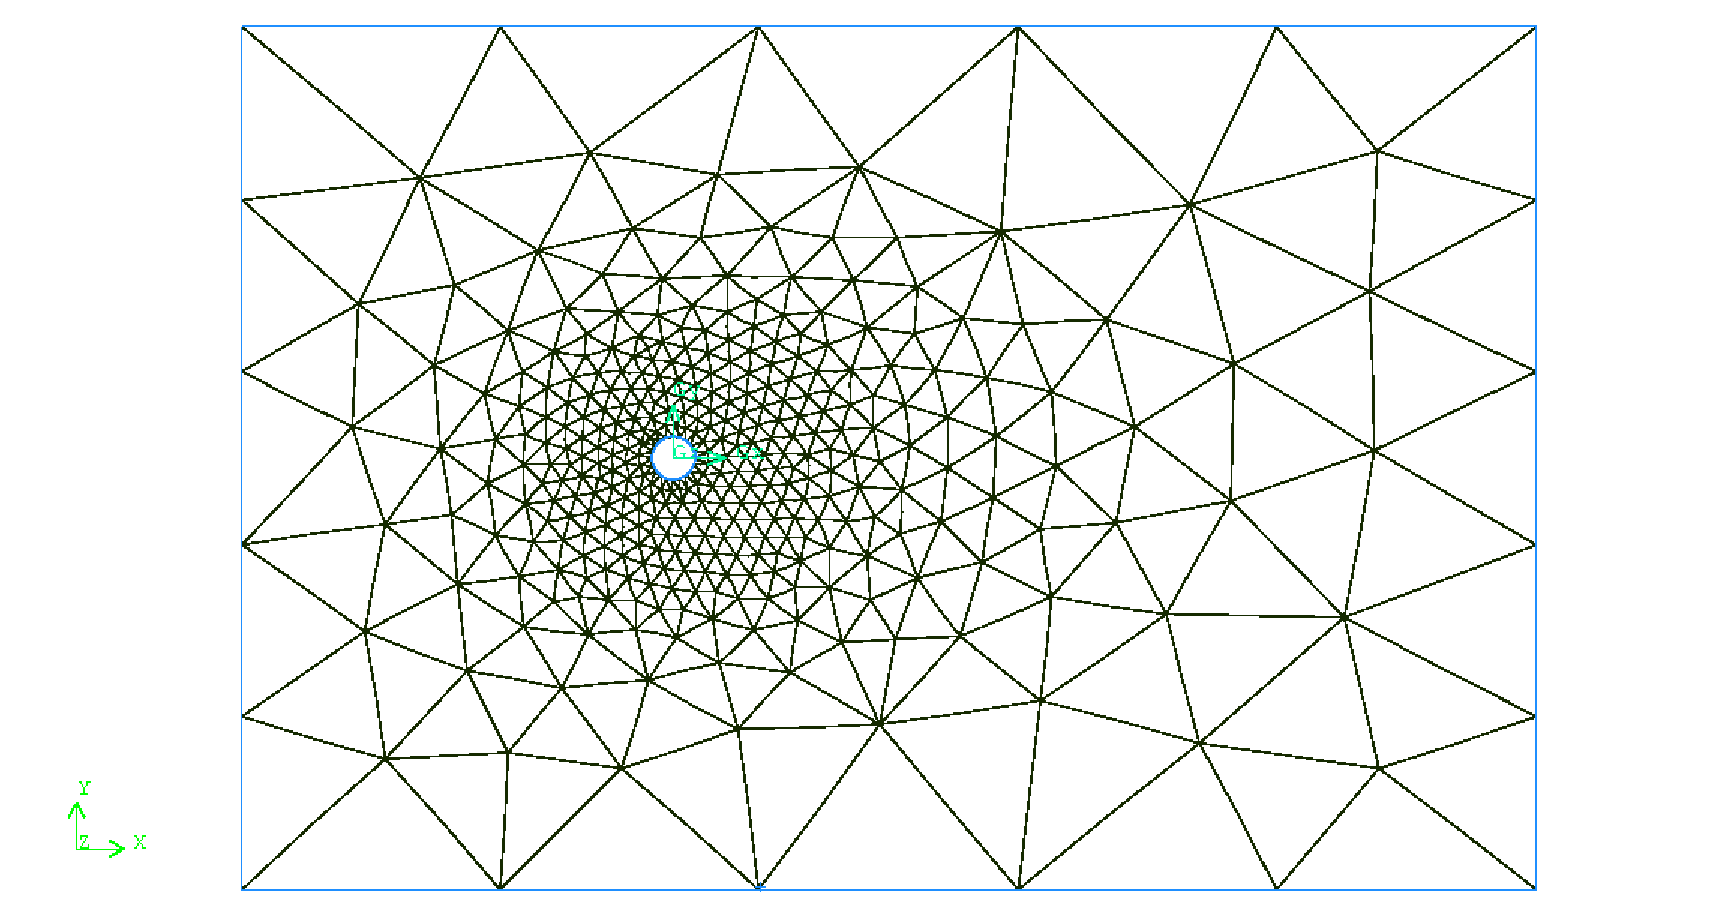
\includegraphics[width=0.55\textwidth]{\lfsdir/figs/MESH2.eps}
}
\hfill
\subfloat[Close-up view \label{fig:mesh_close}]{%
\centering
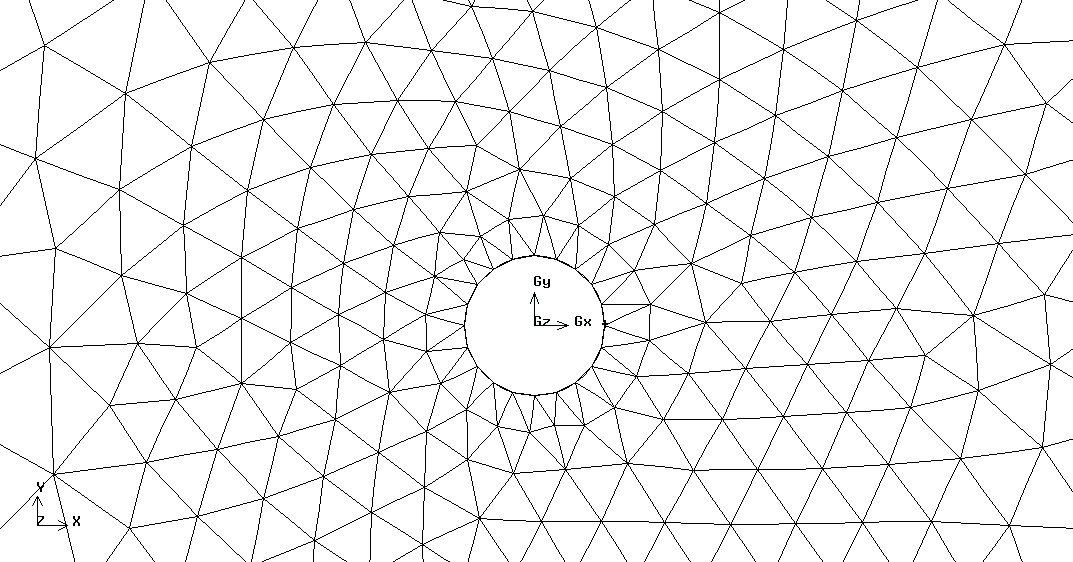
\includegraphics[width=0.55\textwidth]{\lfsdir/figs/MESH_CLOSE.png}
}
\caption{Unstructured, coarse mesh of a circular cylinder with $714$ triangular elements. Elements adjacent to the cylinder have quadratic edges.}
\label{fig:meshes}

\end{figure*}

\subsection{Flow Around a Circular Cylinder, $\bf Re =  10^6, Ma = 0.2$}
This was the first simulation performed after implementing the filters in \gls{hf}, so the \gls{gpu} implementation was not available then. The time-stepping scheme used here is simply forward Euler.

Figure \ref{fig:Ma0.2Re1e6_Ma} shows ``pretty pictures" resulting from the simulation. A video of this simulation is linked \href{https://youtu.be/b6kx8-jrK6Q}{here}.

It is interesting to note that there is a very dissipative form of vortex shedding occurring. The wake region is long, as in lower \gls{re}-number cases.

The simulation remained stable throughout and no human intervention was performed while it was occurring, from the start in uniform flow to the moment it was stopped.

From this experiment, it is unclear what portion of the numerical dissipation arises from the coarse discretization and what portion is due to the filtering operation.

This case demonstrates that the stabilization strategy can work well in cases where the mesh is improperly refined: they stabilize the solution and preserve the boundary conditions.

\begin{figure*}
\hspace{-1cm}
\subfloat[Full view \label{fig:Ma0_2Re1e6_Ma_far}]{%
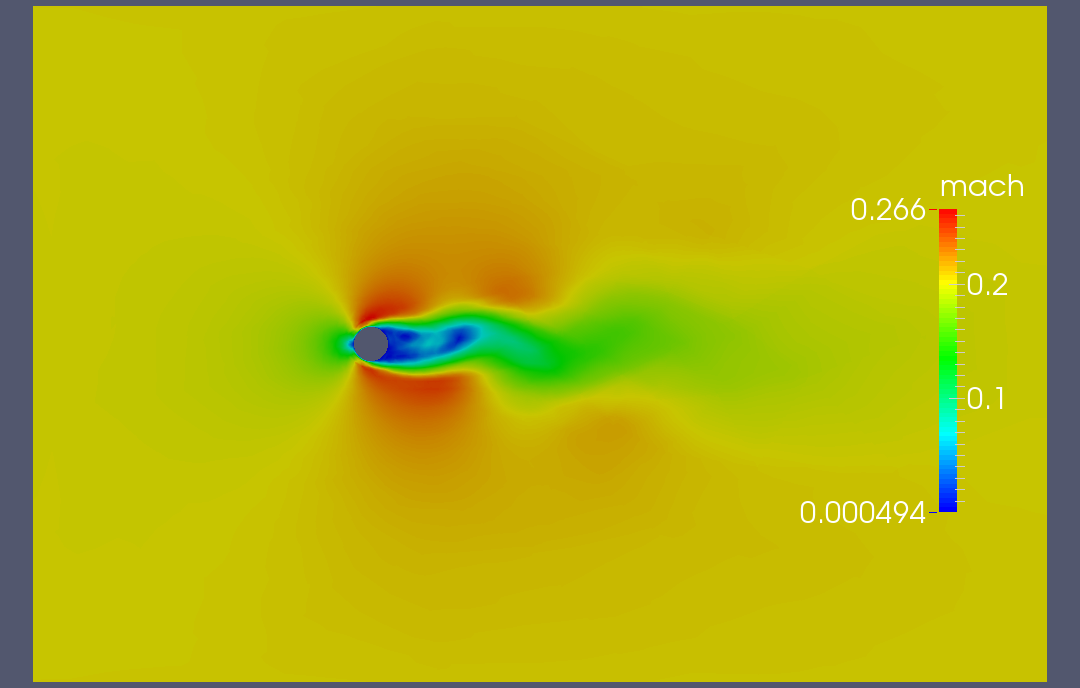
\includegraphics[width=0.55\textwidth]{\lfsdir/figs/Ma0_2--Re1e6_Ma.png}
}
\hfill
\subfloat[Close-up view \label{fig:Ma0_2Re1e6_Ma_close}]{%
\centering
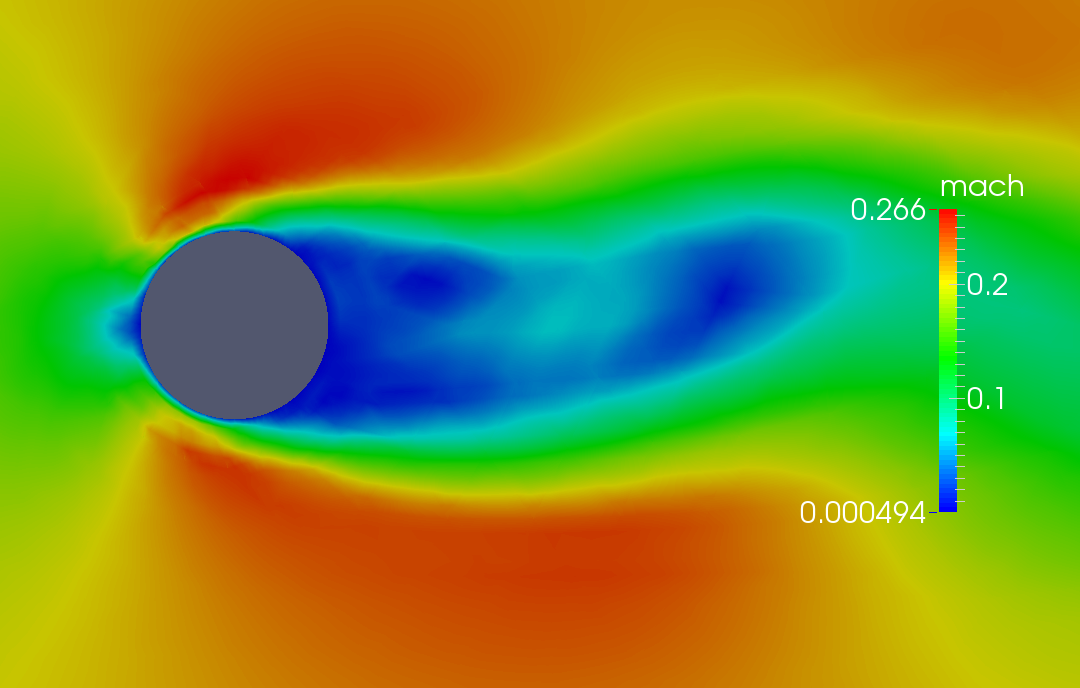
\includegraphics[width=0.55\textwidth]{\lfsdir/figs/Ma0_2--Re1e6_Ma_closeup.png}
}
\caption{Flow past a cylinder. $\Re = 1e6, \Ma = 0.2, p = 4$}
\label{fig:Ma0.2Re1e6_Ma}

\end{figure*}

\subsection{High Reynolds Number, Flow Around a Circular Cylinder, $\bf Re = 10^6, Ma = 0.077$}
This was the first simulation performed using \gls{gpu}s. The lower \gls{ma} case was of interest, as \gls{hf} had not been able to run full simulations of flows with \gls{ma}$< 0.2$.

Figure \ref{fig:Ma0.077Re1e6_Ma} shows the colorful results for this case. Once again, the boundary conditions are satisfied and the simulation is stabilized without further intervention. The same time-step size was used as in the previous case in order to leave as many parameters as possible unchanged.

A video of this simulation is linked \href{https://youtu.be/EymTVFzyPcA}{here} in real-time, and \href{https://youtu.be/8ZH349_GRUA}{here} at 0.1$\times$. A feature of these simulations that can only be appreciated by watching the linked videos is that the filters have a visible effect on the regions where aliasing and instabilities are expected: the rear part of the cylinder and the boundary layer. However, even though the filters are being applied everywhere, smooth, well-resolved regions of the flow look unchanged. To what extent the smooth regions remain unchanged has not been quantified.

\begin{figure*}
\hspace{-1cm}
\subfloat[Full view \label{fig:Ma0_077Re1e6_Ma_far}]{%
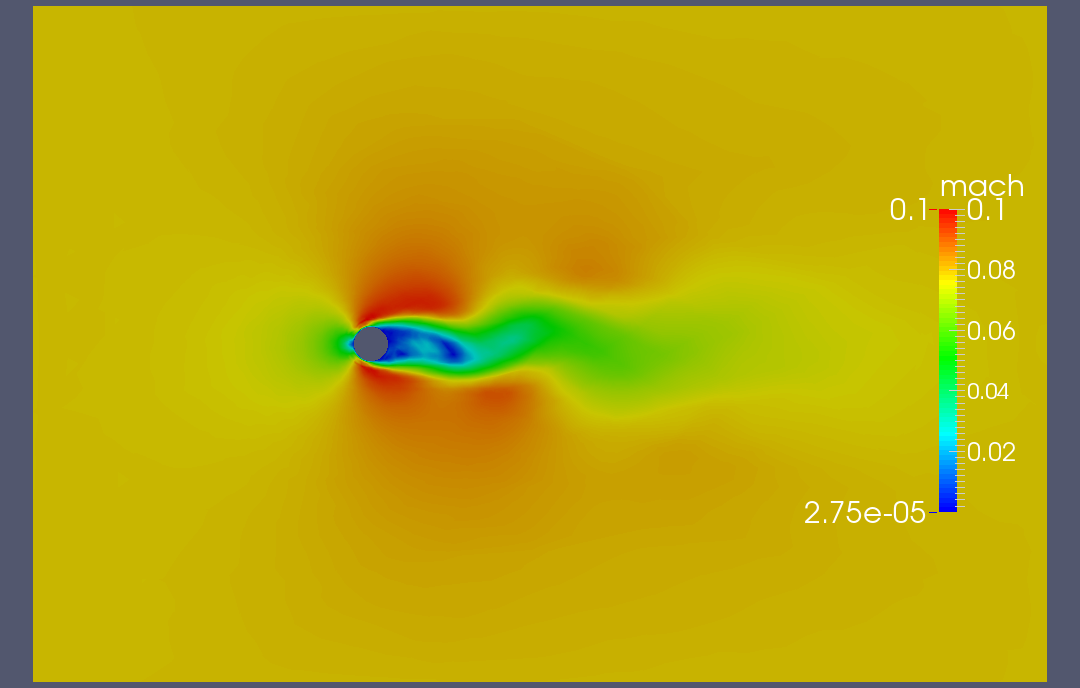
\includegraphics[width=0.55\textwidth]{\lfsdir/figs/Ma0_077--Re1e6_Ma.png}
}
\hfill
\subfloat[Close-up view \label{fig:Ma0_077Re1e6_Ma_close}]{%
\centering
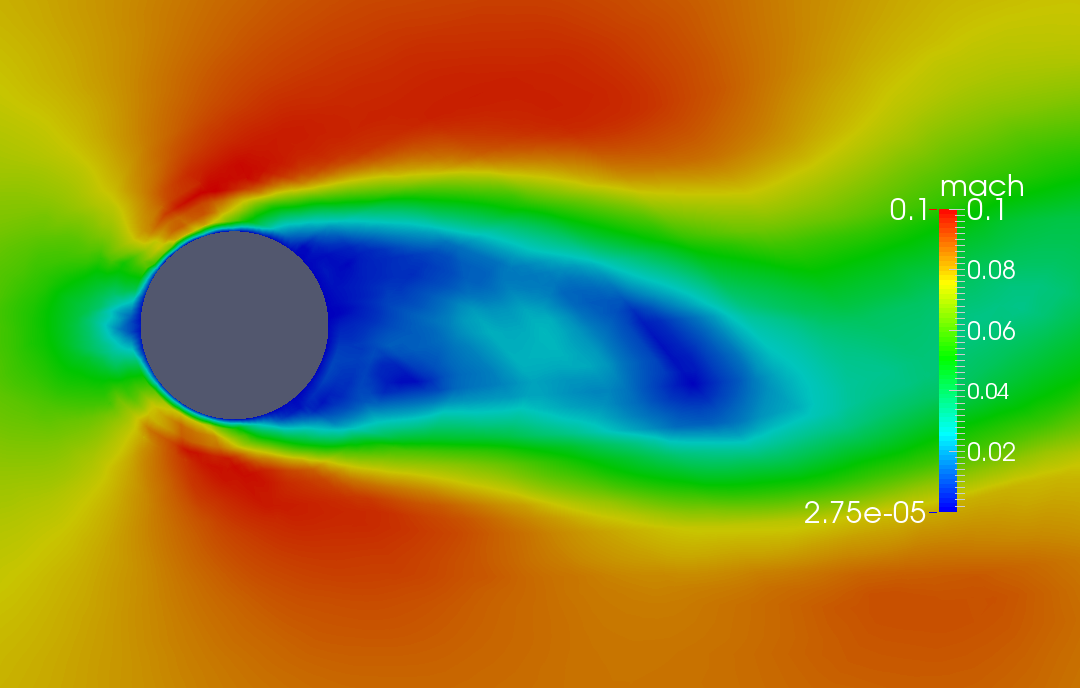
\includegraphics[width=0.55\textwidth]{\lfsdir/figs/Ma0_077--Re1e6_Ma_closeup.png}
}
\caption{Flow past a cylinder. \gls{re}$= 1e6$, \gls{ma} $= 0.077, p = 4$}
\label{fig:Ma0.077Re1e6_Ma}

\end{figure*}

%\subsection{High Reynolds Number, Flow Around a Circular Cylinder, $\bf Re = 10^6, Ma = 0.85$}

\begin{figure*}
\hspace{-1cm}
\subfloat[Full view \label{fig:Ma0_87Re1e6_Ma_unstable_far}]{%
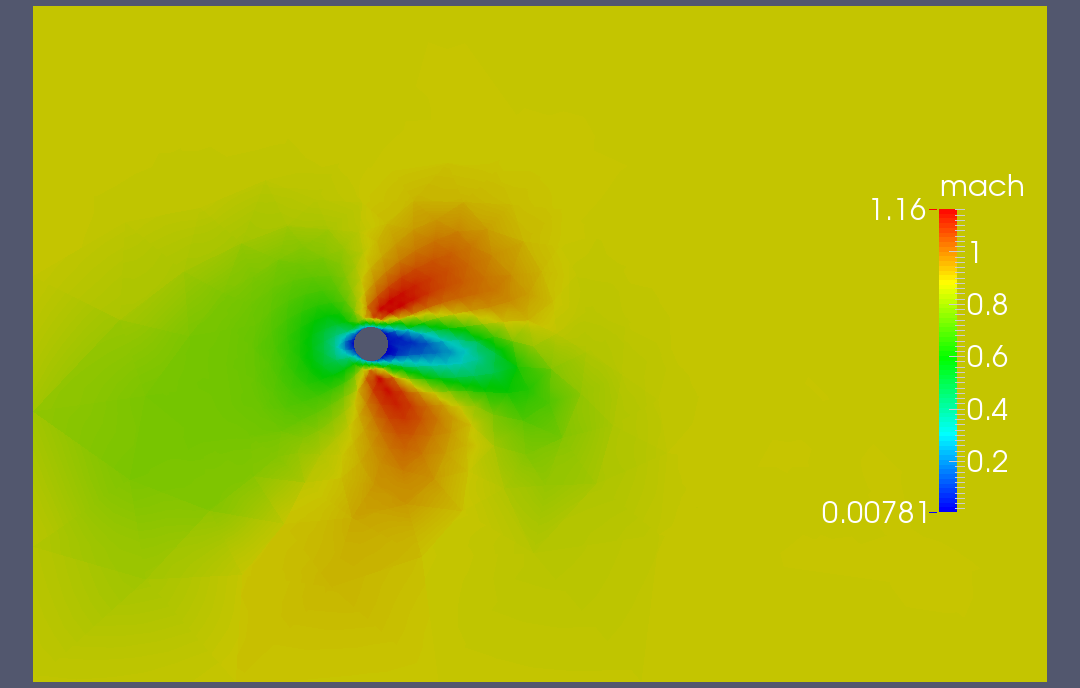
\includegraphics[width=0.55\textwidth]{figs/Ma0_87--Re1e6_Ma.png}
}
\hfill
\subfloat[Close-up view \label{fig:Ma0_87Re1e6_Ma__unstable_close}]{%
\centering
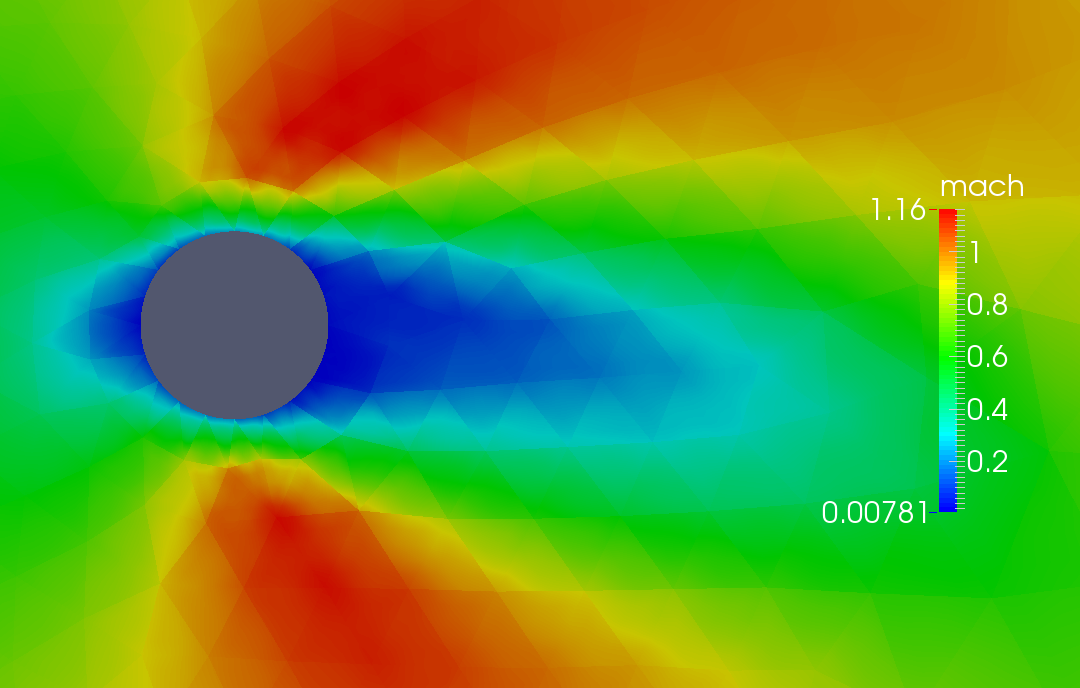
\includegraphics[width=0.55\textwidth]{figs/Ma0_87--Re1e6_Ma_closeup.png}
}

\hspace{-1cm}
\subfloat[Close-up view \label{fig:Ma0_87Re1e6_P__unstable}]{%
\centering
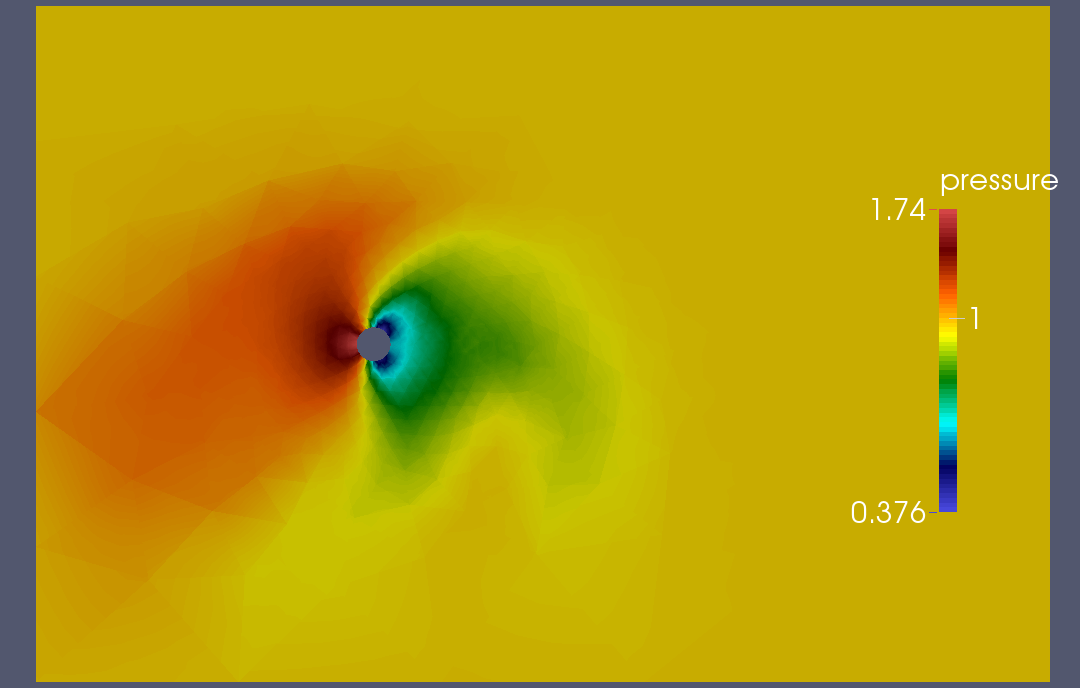
\includegraphics[width=0.55\textwidth]{figs/Ma0_87--Re1e6_P.png}
}
\hfill
\subfloat[Close-up view \label{fig:Ma0_87Re1e6_P__unstable_close}]{%
\centering
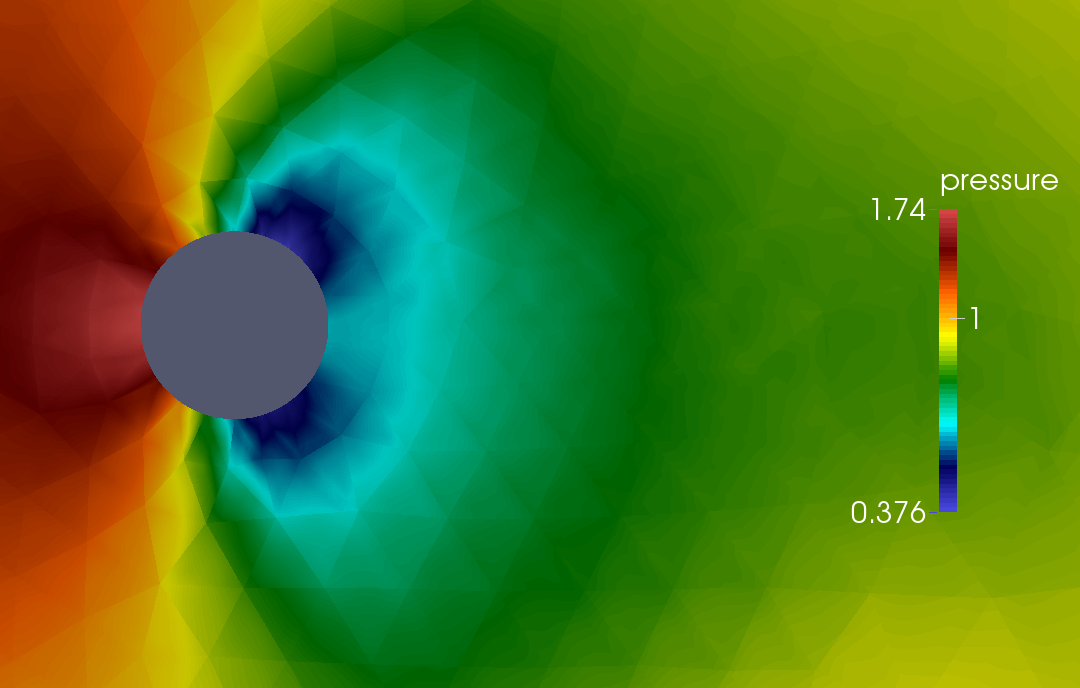
\includegraphics[width=0.55\textwidth]{figs/Ma0_87--Re1e6_P_closeup.png}
}
\caption{$\Re = 1e6, \Ma = 0.87, p = 4$}
\label{fig:Ma0.87Re1e6_unstable_Ma}
\end{figure*}

\subsection{High Reynolds Number, Flow Around a Circular Cylinder, $\bf Re = 10^6, Ma = 0.87$}

This case encompases all potential sources of instabilities in a high-order solver: poor resolution, aliasing, and sharp gradients. Figure \ref{fig:Ma0.87Re1e6} shows plots of the solution. The simulation shows a clear un-physical asymmetry due to the coarseness of the mesh. Nevertheless, the no-slip boundary conditions are being satisfied and the shock is present. 

Because of the coarseness of the mesh and the high-gradients present in the solution, quite a lot of filtering had to occur. This forced the flow to a ``steady state" and shown in the Residual and $C_D$ plots in Figure \ref{fig:Ma0.87Re1e6_history}.

\begin{figure*}
\hspace{-1cm}
\subfloat[Full view \label{fig:Ma0_87Re1e6_Ma_far}]{%
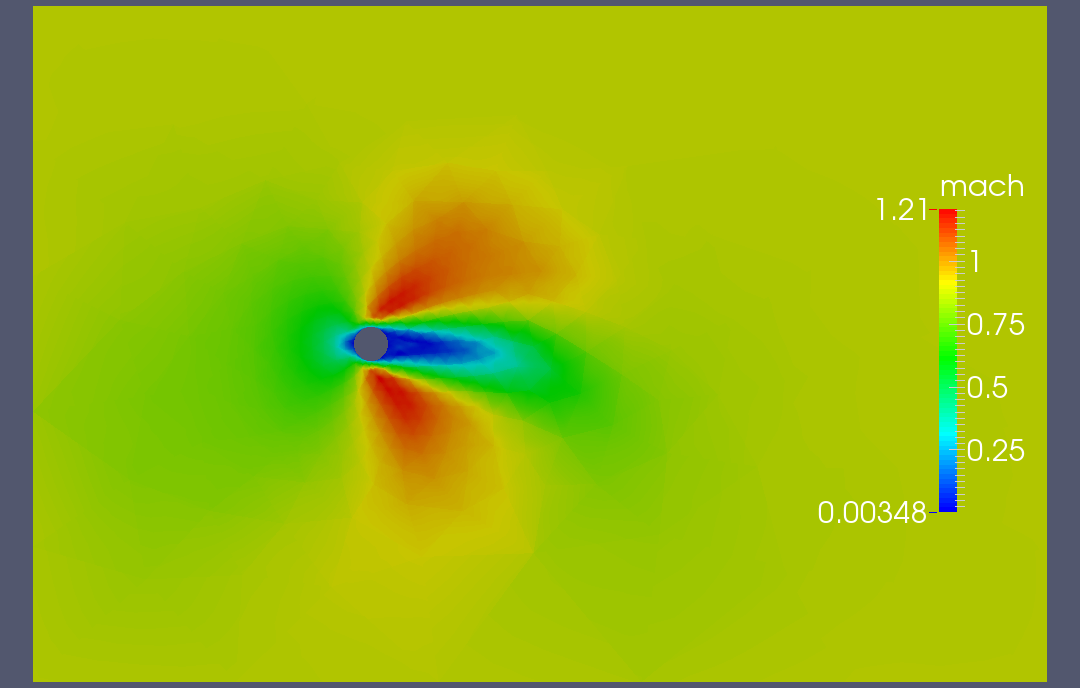
\includegraphics[width=0.55\textwidth]{\lfsdir/figs/Ma0_87--Re1e6_Ma_stable.png}
}
\hfill
\subfloat[Close-up view \label{fig:Ma0_87Re1e6_Ma_close}]{%
\centering
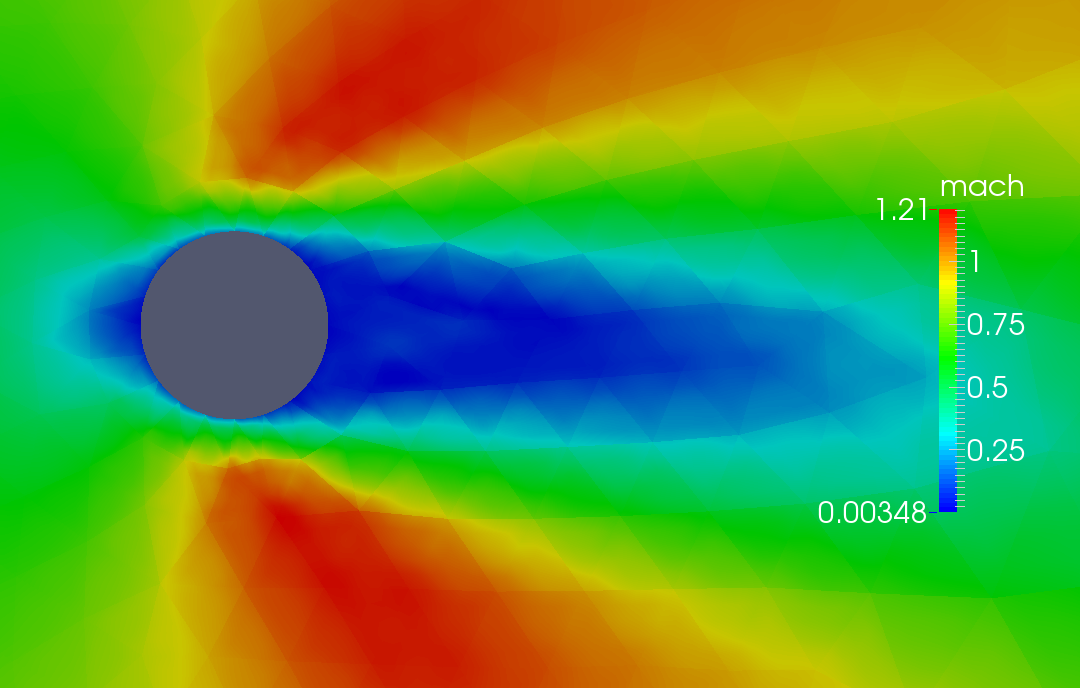
\includegraphics[width=0.55\textwidth]{\lfsdir/figs/Ma0_87--Re1e6_Ma_stable_closeup.png}
}

\hspace{-1cm}
\subfloat[Full view \label{fig:Ma0_87Re1e6_P_stable}]{%
\centering
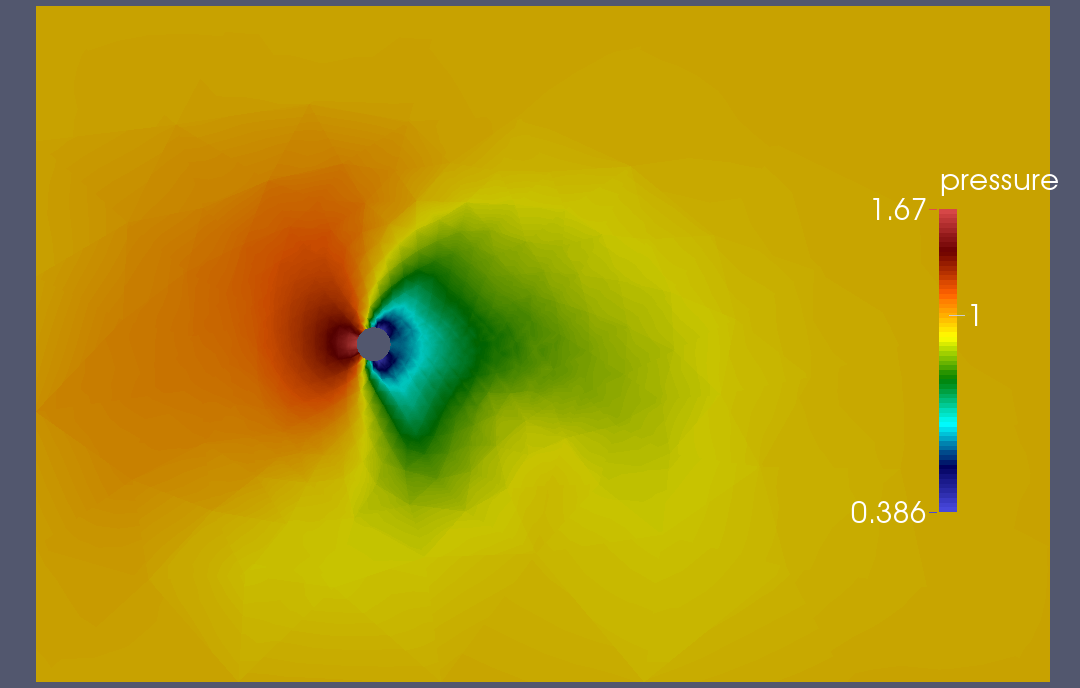
\includegraphics[width=0.55\textwidth]{\lfsdir/figs/Ma0_87--Re1e6_P_stable.png}
}
\hfill
\subfloat[Close-up view \label{fig:Ma0_87Re1e6_P_stable_close}]{%
\centering
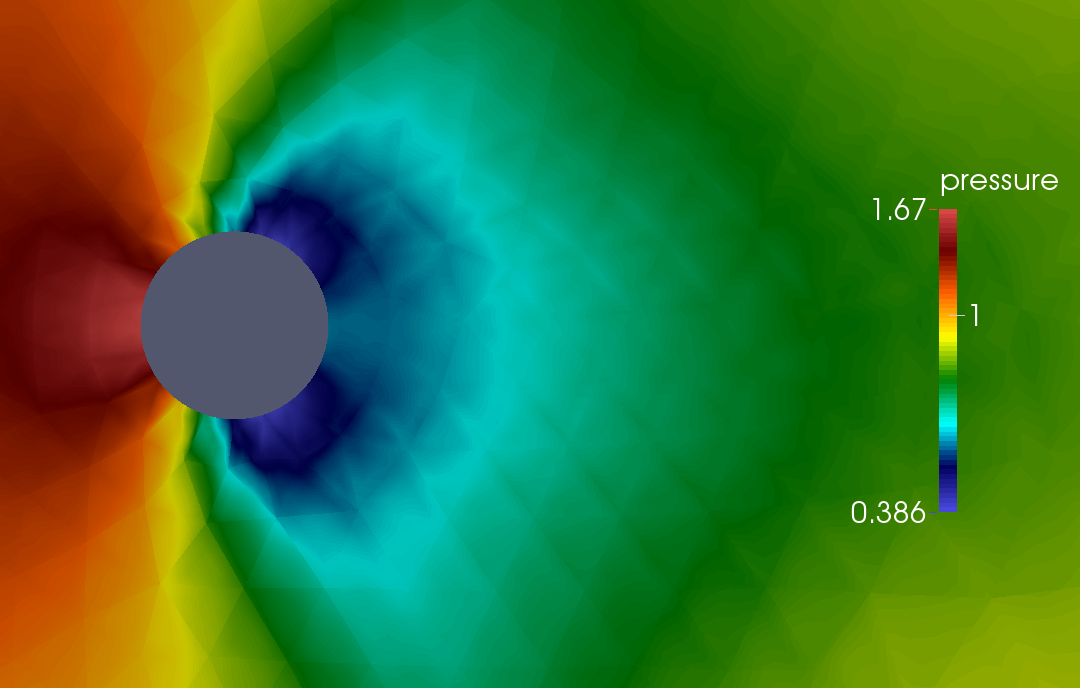
\includegraphics[width=0.55\textwidth]{\lfsdir/figs/Ma0_87--Re1e6_P_stable_closeup.png}
}
\caption{Flow past a cylinder. \gls{re}$= 1e6$, \gls{ma} $= 0.87, p = 4$}
\label{fig:Ma0.87Re1e6}

\end{figure*}

Values of $C_D$ and residual history are shown in Figure \ref{fig:Ma0.87Re1e6_history}. The value of drag ``converges" after time-step $1.846e6$. The residual in the energy conservation equation also ``converges" to a zig-zag pattern after this iteration. Figure \ref{fig:rhoE_res_history} shows the energy residual in the last few thousand time-steps. The sharp decrease in residual magnitude reveals the time-steps at which the filter is being applied.

\begin{figure*}
\subfloat[Drag coefficient history over entire simulation run. ``Steady state" is reached at time-step $1.846e6$. \label{fig:cd_history}]{%
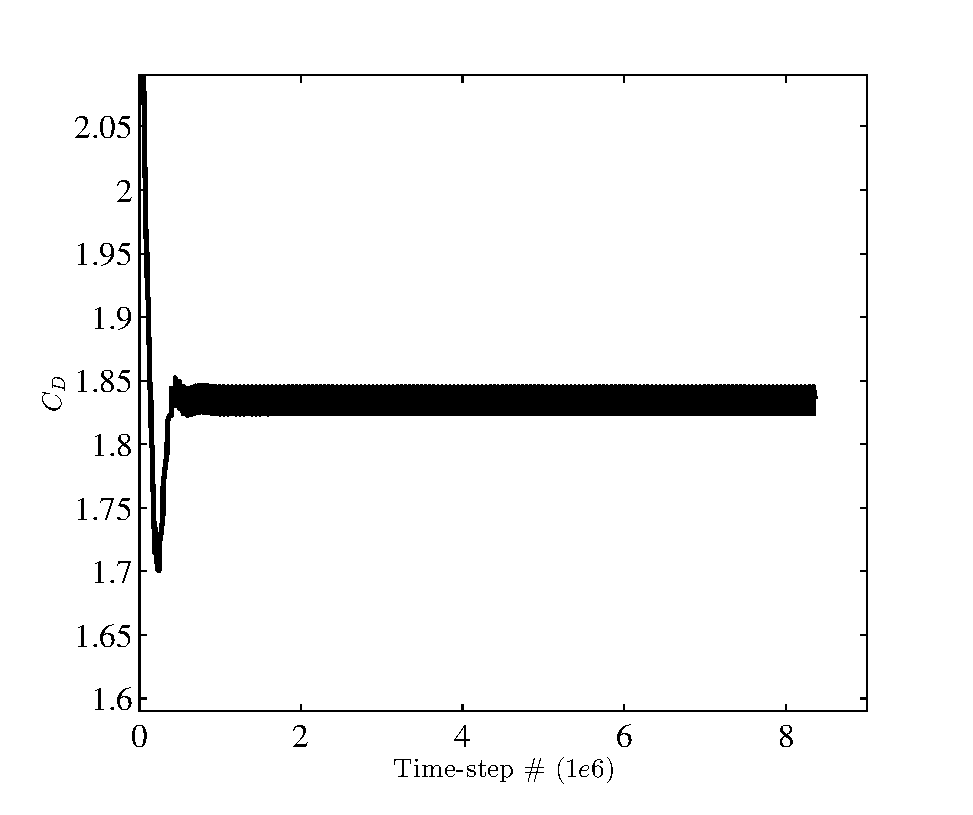
\includegraphics[width=0.55\textwidth]{\lfsdir/figs/unstable_c_d.eps}
}
\hfill
\subfloat[Energy residual history over the last few thousand time-steps \label{fig:rhoE_res_history}]{%
\centering
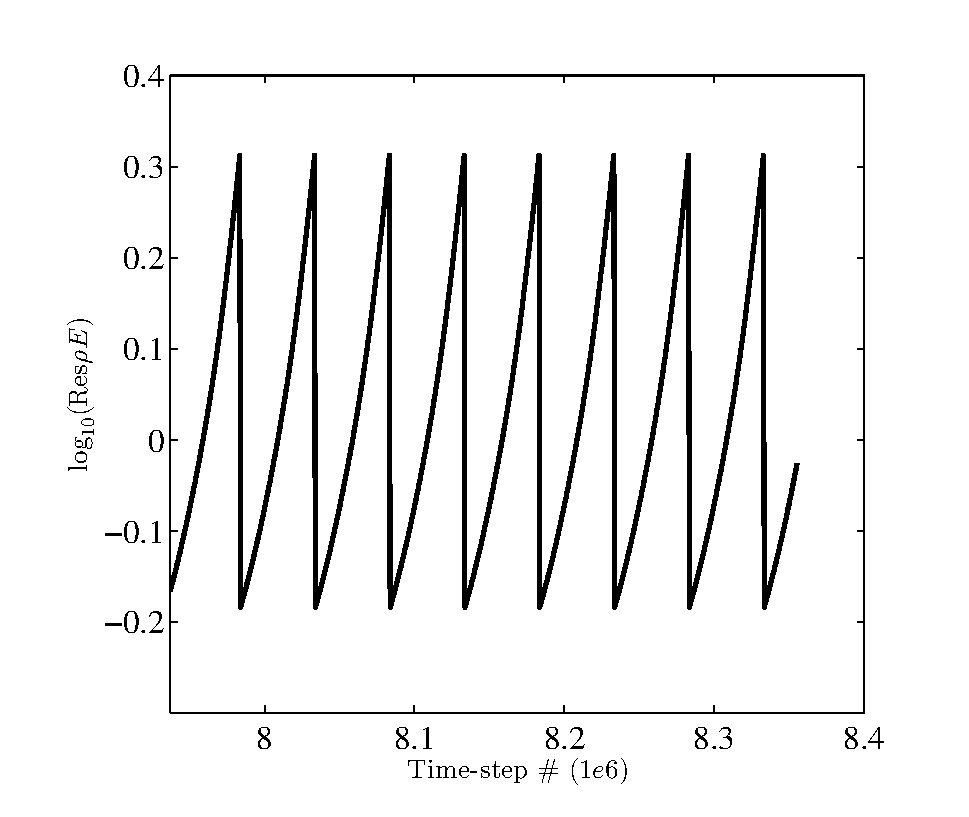
\includegraphics[width=0.55\textwidth]{\lfsdir/figs/unstable_rhoE_res.eps}
}
\caption{History of $C_D$ and energy residual of simulation in Figure \ref{fig:Ma0.87Re1e6}}
\label{fig:Ma0.87Re1e6_history}

\end{figure*}

\subsection{High Reynolds Number, Flow Around a Circular Cylinder, $\bf Re = 10^6, Ma = 0.0077$, less-coarse mesh}
This case was run with the more refined mesh seen in Figure \ref{fig:meshes2}. This mesh is still coarse for standard turbulent computations. It is interesting to note that the predicted $C_D = 1.18$ and $\mathrm{St} = 0.20$ match experimental results for \gls{re}$= 2e2$. This phenomenon could imply that the grid of the stabilized simulation determines the effective Reynolds number being simulated.

A real-time video of this simulation is linked \href{https://youtu.be/XSzWPn2fZ90}{here} for Mach contours, and \href{https://youtu.be/_zIbZgHjepY}{here} for vorticity strength contours. The filters stabilized this almost-incompressible simulation without a problem.


\begin{figure*}
\hspace{-1cm}
\subfloat[Full mesh view \label{fig:mesh2}]{%
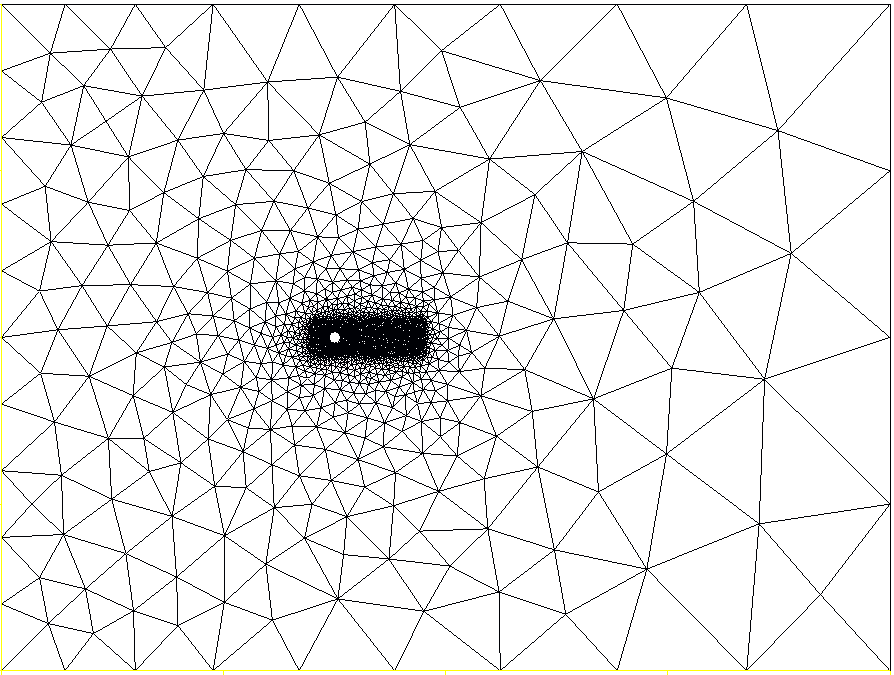
\includegraphics[width=0.55\textwidth]{\lfsdir/figs/cylinder_fine_v2.png}
}
\hfill
\subfloat[Close-up view \label{fig:mesh2_close}]{%
\centering
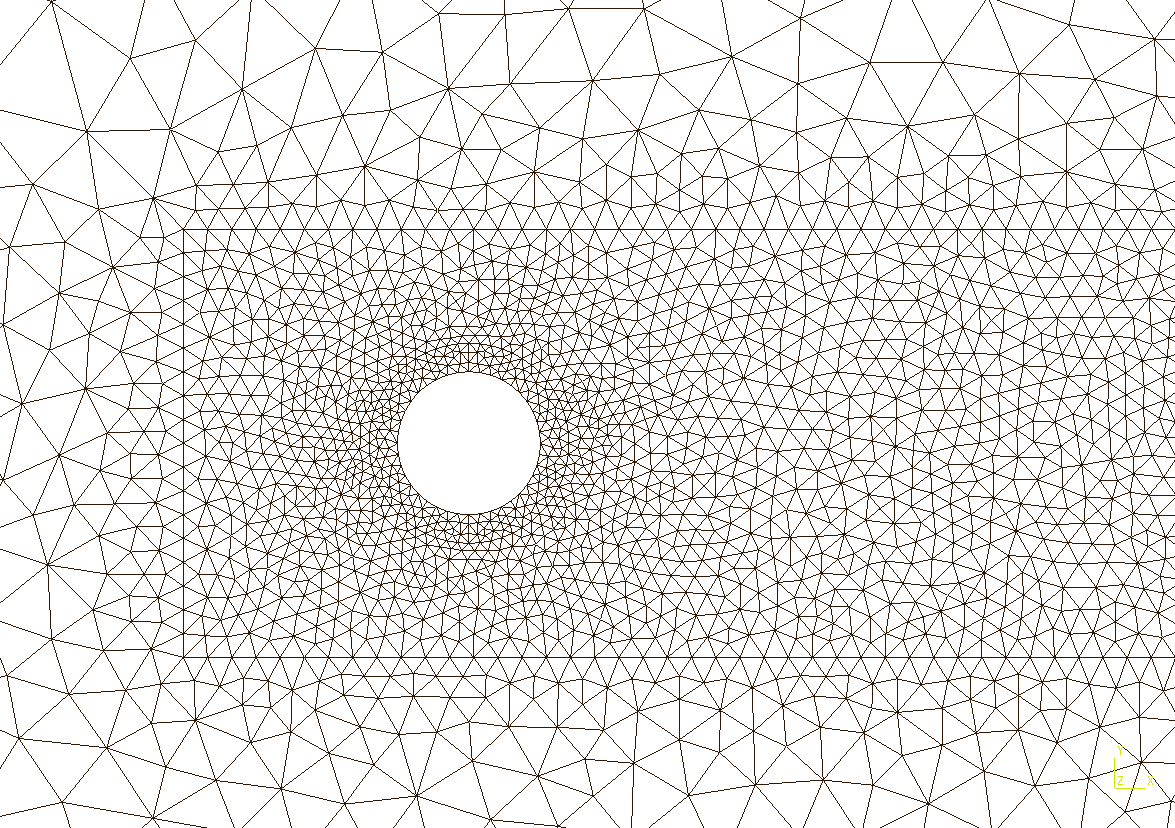
\includegraphics[width=0.55\textwidth]{\lfsdir/figs/mesh_closeup_2.png}
}
\caption{Unstructured, coarse mesh of a circular cylinder with 5,616 triangular elements. Elements adjacent to the cylinder have quadratic edges.}
\label{fig:meshes2}

\end{figure*}


\begin{figure*}
\hspace{-1cm}
\subfloat[Full view \label{fig:Ma0_0077Re1e6_Ma_far}]{%
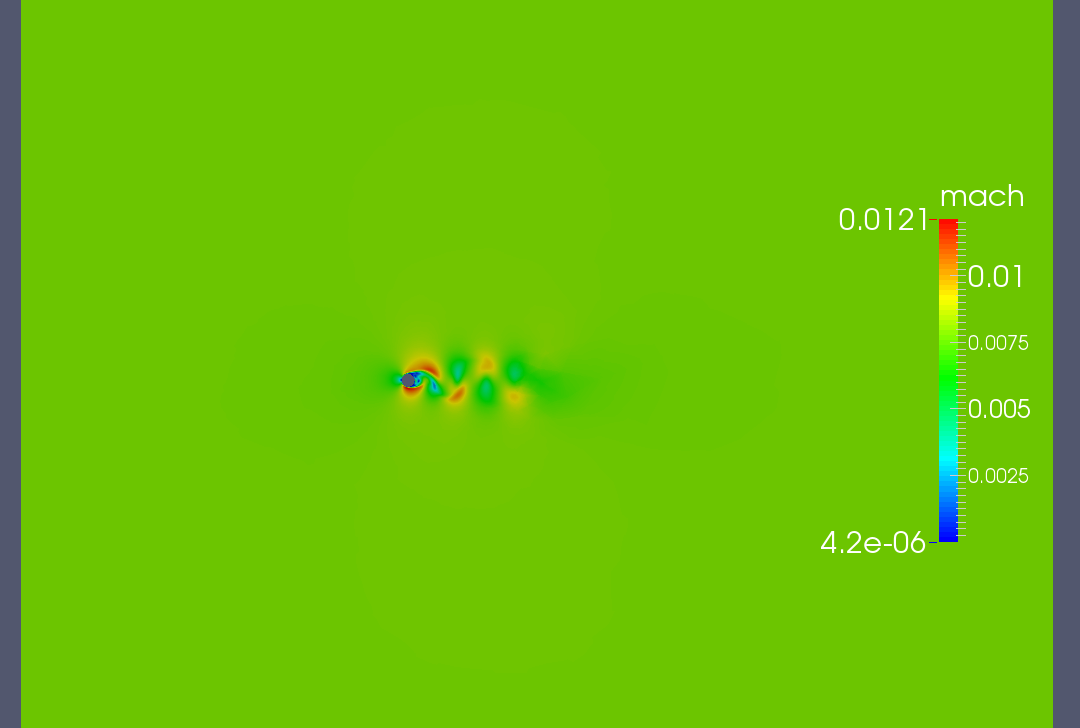
\includegraphics[width=0.55\textwidth]{\lfsdir/figs/Ma0_0077--Re1e6_Ma.png}
}
\hfill
\subfloat[Close-up view \label{fig:Ma0_0077Re1e6_Ma_close}]{%
\centering
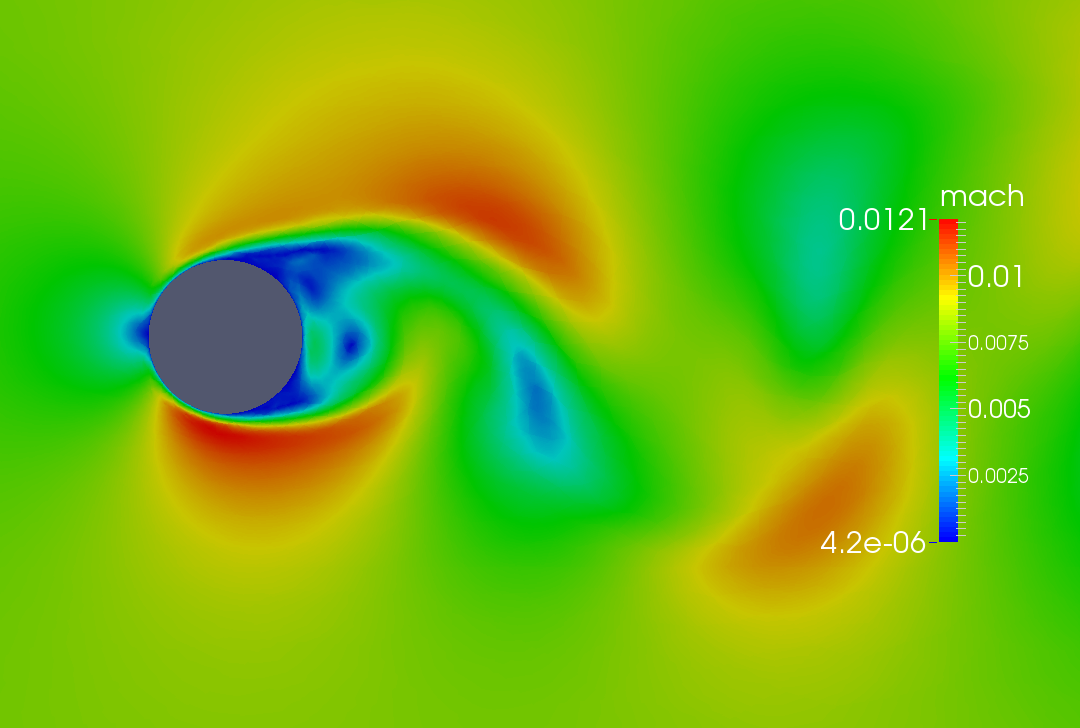
\includegraphics[width=0.55\textwidth]{\lfsdir/figs/Ma0_0077--Re1e6_Ma_closeup.png}
}
\caption{Flow past a cylinder. \gls{re}$= 1e6$, \gls{ma} $= 0.0077, p = 4$}
\label{fig:Ma0.0077Re1e6_Ma}

\end{figure*}




\vspace{.20in}

\section{Conclusion}
\label{sec:conclusion}

We have suggested a formulation of \gls{lfs} filters for the stabilization of \gls{ns} solvers for unstructured grids that use a Finite Element Method-based approach to achieve high order spatial discretizations. This includes \gls{dg}, \gls{sd}, Spectral Element, and \gls{fr} methods. The filtering operation can be performed at individual elements and maintains a local stencil by using the element's solution and boundary values. This makes their implementation highly parallelizable.

The filters have been developed with the desired properties shown in Section \ref{sec:lfs_properties}. In essence, the filters have a spectral interpretation and satisfy boundary conditions asymptotically. The computational cost of applying a filtering operation to a single element is two small matrix multiplications. This low cost plus the compact stencil makes the \gls{lfs} filters a good alternative to using artificial dissipation. The main advantage of \gls{lfs} filters over artificial dissipation is that no modification needs to be made to the partial differential equations being solved.

We have shown by implementing the \gls{lfs} filters in \gls{hf} that little to no tuning is necessary to achieve stability in cases where instability is expected: coarse grids, high-\gls{re} flows, high-\gls{ma} flows, and low-\gls{ma} flows. In all cases, the filters preserved the boundary conditions, did not introduce visible flow anomalies, and allowed the flow to develop its natural features. The summary of results can be seen in Table \ref{table:results}.

Because the filter has a physical interpretation, \gls{sgs} modeling could be done with the classical physical arguments. A similar type of filter has been used by Lodato\cite{lodato2014structural} in the \gls{sd} scheme to do \gls{sgs} modeling rather than to stabilize the solution.

The unexpected finding that the filters could bring simulations in very coarse meshes to a pseudo-steady state opens up the possibility of using the \gls{lfs} filters as part of a pre-conditioning strategy or to start flow simulations from conditions more developed than uniform flow.

All algorithms are publicly available in the \gls{hf} \href{https://github.com/HiFiLES/HiFiLES-solver}{repository} under the branch ``\gls{lfs}-filters". The filters have been fully implemented for \gls{gpu}/CPU computations for triangular grids only.

%The results seen in \cite{asthana2014} are very promising, given that a double shock 2D simulation with $9^\text{th}$ order of accuracy are possible. We have recently submitted an article\cite{asthana2014} to JCP showing the promising results. Due to time constraints (the article was submitted on November 12, 2014), we have not produced results different to those in the article, but expect to have excellent results in the final version.
%
\vspace{.10in}

\section{Future Work}
\label{sec:future_work}
Implementation in 3D elements is straightforward and shall be the immediate course of action. 3D high-\gls{re} simulations had not been possible in \gls{hf} and it is expected stabilization with \gls{lfs} filters will enable them.

So far in all simulations the filters are acting on all elements in the domain with a pre-determined frequency. A more surgical approach to filtering is needed. As shown by Lv et al.~\cite{lv2015entropy}, localized and selective direct solution manipulation (limiting by multiplying the solution by a scalar while preserving the average within an element) can preserve the overall order of accuracy. The implementation of an aliasing/shock sensor is in order. Because the filters appear to have little effect on regions where the solution is well resolved, it is acceptable if the sensor is too conservative. The sensor proposed by Persson et al.~\cite{persson2006sub} for general elements and by Sheshadri et al.~\cite{Sheshadri2014} for tensor-product elements are prime candidates.

The filters are modifying all conservation variables within an element, and very likely key flow quantities like entropy and pressure are being disturbed. This disturbance needs to be quantified.

To prove the usefulness of the \gls{lfs} filters in a challenging simulation environment, it will be essential to assess their performance in a grid refined properly for the case at hand.
\vspace{-.20in}
